\documentclass[a4paper,11pt,twoside]{ThesisStyle}
\usepackage{etex}

\usepackage{fancyhdr}

\usepackage[left=1.4in,right=1.3in,top=1.1in,bottom=1.1in,includefoot,includehead,headheight=13.6pt]{geometry}

% Table of contents for each chapter
\usepackage[nottoc, notlof, notlot]{tocbibind}
\usepackage{minitoc}
\setcounter{minitocdepth}{2}
\mtcindent=15pt

% Glossary / list of abbreviations
\usepackage[intoc]{nomencl}
\renewcommand{\nomname}{List of Abbreviations}
\makenomenclature

%%%%%%%%%%%%%%%%%%%%%%%%%%%%%%%%%%%%%%%%%%%%%%%%%%%%%%%%%%%%%%%%%%
% ToDo Code
%%%%%%%%%%%%%%%%%%%%%%%%%%%%%%%%%%%%%%%%%%%%%%%%%%%%%%%%%%%%%%%%%%
\usepackage{xargs}
\newcommandx{\unsure}[2][1=]{\todo[linecolor=red,backgroundcolor=red!25,bordercolor=red,#1]{#2}}
\newcommandx{\change}[2][1=]{\todo[linecolor=blue,backgroundcolor=blue!25,bordercolor=blue,#1]{#2}}
\newcommandx{\info}[2][1=]{\todo[linecolor=green,backgroundcolor=green!25,bordercolor=green,#1]{#2}}
\newcommandx{\improvement}[2][1=]{\todo[linecolor=magenta,backgroundcolor=magenta!25,bordercolor=magenta,#1]{#2}}
\newcommandx{\fix}[2][1=]{\todo[linecolor=red,backgroundcolor=red!25,bordercolor=red,#1]{#2}}

%%%%%%%%%%%%%%%%%%%%%%%%%%%%%%%%%%%%%%%%%%%%%%%%%%%%%%%%%%%%%%%%%%
% PDF Code
%%%%%%%%%%%%%%%%%%%%%%%%%%%%%%%%%%%%%%%%%%%%%%%%%%%%%%%%%%%%%%%%%%

\usepackage{ifpdf}

\ifpdf
  \usepackage[pdftex]{graphicx}
  \DeclareGraphicsExtensions{.jpg}
  \usepackage[hyperindex=true]{hyperref}
\else
  \usepackage{graphicx}
  \DeclareGraphicsExtensions{.ps,.eps}
  \usepackage[dvipdfm,hyperindex=true]{hyperref}
\fi

\graphicspath{{.}{images/}}

% definitions.

\setcounter{secnumdepth}{3}
\setcounter{tocdepth}{2}

% Some useful commands and shortcut for maths:  partial derivative and stuff

\usepackage [table]{xcolor}

\newcommand{\pd}[2]{\frac{\partial #1}{\partial #2}}
\def\abs{\operatorname{abs}}
\def\argmax{\operatornamewithlimits{arg\,max}}
\def\argmin{\operatornamewithlimits{arg\,min}}
\def\diag{\operatorname{Diag}}
\newcommand{\eqRef}[1]{(\ref{#1})}

%%%%%%%%%%%%%%%%%%%%%%%%%%%%%%%%%%%%%%%%%%%%%%%%%%%%%%%%%%%%%%%%%%
% Fancy Header Style Options
%%%%%%%%%%%%%%%%%%%%%%%%%%%%%%%%%%%%%%%%%%%%%%%%%%%%%%%%%%%%%%%%%%

% Sets fancy header and footer
\pagestyle{fancy}
% Delete current footer settings
\fancyfoot{}
% Page number (boldface) in left on even
\fancyhead[LE,RO]{\bfseries\thepage}
% pages and right on odd pages
\fancyhead[RE]{\small\bfseries\nouppercase{\leftmark}}      % Chapter in the right on even pages
\fancyhead[LO]{\small\bfseries\nouppercase{\rightmark}}     % Section in the left on odd pages
\let\headruleORIG\headrule
\renewcommand{\headrule}{\color{black} \headruleORIG}
\renewcommand{\headrulewidth}{1.0pt}
\arrayrulecolor{black}

\fancypagestyle{plain}{
  \fancyhead{}
  \fancyfoot{}
  \renewcommand{\headrulewidth}{0pt}
}

% Clear Header Style on the Last Empty Odd pages
\makeatletter

\def\cleardoublepage{\clearpage\if@twoside \ifodd\c@page\else%
  \hbox{}%
  \thispagestyle{empty}%              % Empty header styles
  \newpage%
  \if@twocolumn\hbox{}\newpage\fi\fi\fi}

\makeatother

%%%%%%%%%%%%%%%%%%%%%%%%%%%%%%%%%%%%%%%%%%%%%%%%%%%%%%%%%%%%%%%%%%%%%%%%%%%%%%%
% Prints your review date and 'Draft Version' (From Josullvn, CS, CMU)
%%%%%%%%%%%%%%%%%%%%%%%%%%%%%%%%%%%%%%%%%%%%%%%%%%%%%%%%%%%%%%%%%%%%%%%%%%%%%%%
\newcommand{\reviewtimetoday}[2]{\special{!userdict begin
    /bop-hook{gsave 20 710 translate 45 rotate 0.8 setgray
      /Times-Roman findfont 12 scalefont setfont 0 0   moveto (#1) show
      0 -12 moveto (#2) show grestore}def end}}

\newenvironment{maxime}[1]
{
\vspace*{0cm}
\hfill
\begin{minipage}{0.5\textwidth}
\hrulefill $\:$ {\bf #1}\\
\it
}
{

\hrulefill
\vspace*{0.5cm}%
\end{minipage}
}

\let\minitocORIG\minitoc
\renewcommand{\minitoc}{\minitocORIG \vspace{1.5em}}

\newenvironment{bulletList}%
{ \begin{list}%
  {$\bullet$}%
  {\setlength{\labelwidth}{25pt}%
   \setlength{\leftmargin}{30pt}%
   \setlength{\itemsep}{\parsep}}}%
{ \end{list} }

\newtheorem{definition}{D?finition}
\renewcommand{\epsilon}{\varepsilon}

%%%%%%%%%%%%%%%%%%%%%%%%%%%%%%%%%%%%%%%%%%%%%%%%%%%%%%%%%%%%%%%%%%
% Centered page environment
%%%%%%%%%%%%%%%%%%%%%%%%%%%%%%%%%%%%%%%%%%%%%%%%%%%%%%%%%%%%%%%%%%

\newcommand{\Author}{Ahmad A Assaf}
\newcommand{\Subject}{Enabling Self Service Data Provisioning Through Semantic Enrichment of Data}

\newenvironment{vcenterpage}
{\newpage\vspace*{\fill}\thispagestyle{empty}\renewcommand{\headrulewidth}{0pt}}
{\vspace*{\fill}}
\usepackage{listings}
\hypersetup{
    unicode=false,                        % non-Latin characters in Acrobat?s bookmarks
    pdftoolbar=true,                      % show Acrobat?s toolbar?
    pdfmenubar=true,                      % show Acrobat?s menu?
    pdffitwindow=false,                   % window fit to page when opened
    pdfstartview={FitH},                  % fits the width of the page to the window
    pdftitle={My title},                  % title
    pdfauthor={Author},                   % author
    pdfsubject={Subject},                 % subject of the document
    pdfcreator={Author},                  % creator of the document
    pdfnewwindow=true,                    % links in new window
    colorlinks=true,                      % false: boxed links; true: colored links
    linkcolor=cyan,                       % color of internal links
    citecolor=red,                        % color of links to bibliography
    filecolor=magenta,                    % color of file links
    urlcolor=blue                         % color of external links
}

\newlength{\plarg}
\setlength{\plarg}{16cm}
\newlength{\glarg}
\setlength{\glarg}{17cm}

%%%%%%%%%%%%%%%%%%%%%%%%%%%%%%%%%%%%%%%%%%%%%%%%%%%%%%%%%%%%%%%%%%
% Listings Definitions
%%%%%%%%%%%%%%%%%%%%%%%%%%%%%%%%%%%%%%%%%%%%%%%%%%%%%%%%%%%%%%%%%%
\colorlet{punct}{red!60!black}
\definecolor{background}{gray}{0.97}
\definecolor{delim}{RGB}{20,105,176}

\lstdefinelanguage{json}{
    basicstyle=\small\ttfamily,
    showstringspaces=false,
    breaklines=true,
    frame=lines,
    captionpos=b,
    aboveskip=3mm,
    belowskip=3mm,
    backgroundcolor=\color{white},
    literate=
      {:}{{{\color{punct}{:}}}}{1}
      {,}{{{\color{punct}{,}}}}{1}
      {[}{{{\color{delim}{[}}}}{1}
      {]}{{{\color{delim}{]}}}}{1},
}

\renewcommand{\ttdefault}{pcr}
\lstdefinelanguage{owl} {
  language=xml,
  basicstyle={\footnotesize\ttfamily},
  numbers=none,
  backgroundcolor=\color{white},
  aboveskip=3mm,
  belowskip=3mm,
  showstringspaces=false,
  columns=flexible,
  keywordstyle={\bfseries\color{blue}},
  commentstyle={\color{red}\textit},
  stringstyle=\color{magenta},
  frame=lines,
  breaklines=true,
  breakatwhitespace=true,
  tabsize=4,
  morekeywords={rdf,rdfs,owl},
  moredelim=*[s][\ttfamily]{:}{:} %Newly added line
}

\listfiles

\newcommand\CyrGuillemot{%
  \def\selectguillfont{\fontencoding{OT2}\fontfamily{wncyr}\selectfont}
  \def\guillemotleft{\selectguillfont\symbol{60}}
  \def\guillemotright{\selectguillfont\symbol{62}}
}

\newcommand\PlGuillemot{%
  \def\selectguillfont{\fontencoding{OT4}\fontfamily{cmr}\selectfont}
  \def\guillemotleft{\selectguillfont\symbol{174}}
  \def\guillemotright{\selectguillfont\symbol{175}}
}

\newcommand\LaGuillemot{%
  \def\selectguillfont{\fontencoding{U}\fontfamily{lasy}%
    \fontseries{m}\fontshape{n}\selectfont}
  \def\guillemotleft{\selectguillfont\hbox{\symbol{40}%
    \kern-0.20em\symbol{40}}}
  \def\guillemotright{\selectguillfont\hbox{\symbol{41}%
    \kern-0.20em\symbol{41}}}
}

\newcommand\ECGuillemot{%
  \def\selectguillfont{\fontencoding{T1}\fontfamily{cmr}\selectfont}
  \def\guillemotleft{\selectguillfont\symbol{19}}
  \def\guillemotright{\selectguillfont\symbol{20}}
}

\newcommand\LMGuillemot{%
  \def\selectguillfont{\fontencoding{T1}\fontfamily{lmr}\selectfont}
  \def\guillemotleft{\selectguillfont\symbol{19}}
  \def\guillemotright{\selectguillfont\symbol{20}}
}

\newcommand\CyrGLeft{\CyrGuillemot\guillemotleft}
\newcommand\CyrGRight{\CyrGuillemot\guillemotright}
\newcommand\PlGLeft{\PlGuillemot\guillemotleft}
\newcommand\PlGRight{\PlGuillemot\guillemotright}
\newcommand\LaGLeft{\LaGuillemot\guillemotleft}
\newcommand\LaGRight{\LaGuillemot\guillemotright}
\newcommand\ECGLeft{\ECGuillemot\guillemotleft}
\newcommand\ECGRight{\ECGuillemot\guillemotright}
\newcommand\LMGLeft{\LMGuillemot\guillemotleft}
\newcommand\LMGRight{\LMGuillemot\guillemotright}

\newcolumntype{L}{>{\arraybackslash}m{13cm}}

\newcommand{\algorithmicrequire}{\textbf{Require:}}
\newcommand{\algorithmicensure}{\textbf{Ensure:}}

\usepackage{url}
\usepackage{psfrag}
\usepackage{array,xspace}
\usepackage[FIGTOPCAP]{subfigure}
\usepackage{epsfig,color}
\usepackage {mathpartir,amssymb,stmaryrd,mathtools}
\usepackage{alltt}
\usepackage{amsmath}
\usepackage{multirow}
\usepackage{color}
\usepackage{verbatim}
\usepackage{booktabs}
\usepackage{cases}
\usepackage{wrapfig}
\usepackage{algorithm}
\usepackage{algorithmic}
\usepackage{amssymb}
\usepackage{tabularx}
\usepackage{longtable}
\usepackage{booktabs}
\usepackage{subfigure}
\usepackage{multirow}
\usepackage{easylist}
\usepackage{setspace}
\usepackage{afterpage}
\usepackage{pdflscape}
\usepackage{caption}
\usepackage{xcolor,colortbl}
\usepackage{rotating}
\usepackage[colorinlistoftodos]{todonotes}
\usepackage{fancyhdr}
\usepackage{chngpage}

\usepackage{silence}

\WarningFilter{minitoc(hints)}{W0023}
\WarningFilter{minitoc(hints)}{W0024}
\WarningFilter{minitoc(hints)}{W0028}
\WarningFilter{minitoc(hints)}{W0030}
\WarningFilter{minitoc(hints)}{W0033}

\def\ttbraces{\let\.=\nobreak\chardef\{=`\{\chardef\}=`\}\chardef\|=`\\}

\newcommand{\TODO}[1]{\textcolor{red}{\textbf{[TODO:#1]}}}

\newenvironment{ttbox}{
 \begin{center}\vspace{-.5ex}
     \begin{tabular}{@{}|@{\,}c@{\,}|@{}}
\hline\\[-2ex]
\begin{minipage}[b]{.98\linewidth}
\begin{alltt}\ttbraces\small}
                     {\end{alltt}
     \end {minipage}\\[.3ex]
  \hline
\end{tabular}
\end{center}}

\newcommand{\symb}[1]{\makebox{\it #1}}
% shorthand for various frameworks

\def \proactive {ProActive}
\newcommand{\aspfun}{ASP${}_\text{fun}$\xspace}
\newcommand{\ttt}[1] {\texttt{#1}}


\newenvironment{myitemize}
{\begin{itemize}
\addtolength{\leftskip}{-1.5ex}
\vspace{-.1ex}}
{\end{itemize}\addtolength{\leftskip}{1.5ex}}

\newcommand\rbeta{\to_{\beta}}
\newcommand\rbetastar{{\to_{\beta}^*}}
\newcommand\parbeta{\Rightarrow_{\beta}}
\newcommand\gle{\sqsubseteq}
\newcommand\ttgle{\mbox{\( \gle \)}}
\newcommand\eps{\varepsilon}
\newcommand\eg{e.g.\ }
\newcommand\ie{i.e.\ }
\newcommand\cf{c.f.\ }
\newcommand\etal{{\it et al.} \ }
\newcommand\ttcl{pre\_cl}
\newcommand\ttsp{\mbox{\( sp \)}}
\newcommand\ttwp{\mbox{\( wp \)}}
\newcommand\ttRinv{R\mbox{\( ^{-1} \)}}
\newcommand\oim{\mbox{\(\llparenthesis\)}}
\newcommand\cim{\mbox{\(\rrparenthesis\)}}
\newcommand\imp\Rightarrow
\newcommand\ttrapp{"}

\newcommand\tthash{\mbox{\tt \#}}
\newcommand\ttcirc{\mbox{\( \circ\)}}
\newcommand\ttforall{\mbox{\( \forall \)}}
\newcommand\ttexists{\mbox{\( \exists \)}}
\newcommand\ttequiv{\mbox{\( \equiv \)}}
\newcommand\ttexistsun{\mbox{\( \exists^1 \)}}
\newcommand\ttin{\mbox{\(\in\)}}
\newcommand\ttnin{\mbox{\(\notin\)}}
\newcommand\ttTimes{\mbox{\(\times\)}}
\newcommand\ttalpha{\mbox{\( \alpha \)}}
\newcommand\ttbeta{\mbox{\( \beta \)}}
\newcommand\ttlam{\mbox{\( \lambda \)}}
\newcommand\ttsig{\mbox{\( \sigma \)}}
\newcommand\tteps{\mbox{\( \varepsilon \)}}
\newcommand\ttOmega{\mbox{\( \Omega \)}}
\newcommand\ttpi{\mbox{\( \pi \)}}
\newcommand\ttgam{\mbox{\( \gamma \)}}
\newcommand\ttneg{\mbox{\( \lnot \)}}
\newcommand\ttor{\mbox{\( \lor \)}}
\newcommand\ttwedge{\mbox{\( \land \)}}
\newcommand\ttimp{\mbox{\( \longrightarrow\)}}
\newcommand\ttImp{\mbox{\( \Longrightarrow\)}}
\newcommand\ttfun{\mbox{\( \Rightarrow\)}}
\newcommand\ttssubseteq{\mbox{\( \subseteq\)}}
\newcommand\ttrbeta{\mbox{\( \rbeta\)}}
\newcommand\ttred{\mbox{\( \to_R\)}}
\newcommand\ttuparrow{\mbox{\( \uparrow\)}}
\newcommand\ttfred{\mbox{\( \to_F\)}}
\newcommand\ttored{\mbox{\( \to_O\)}}

\newcommand\ttrbetastar{\mbox{\( \rbetastar\)}}
\newcommand\ttparbeta{\mbox{\( \parbeta\)}}
\newcommand\ttneq{\mbox{\( \neq \)}}
\newcommand\ttbigcup{\mbox{\( \bigcup \)}}
\newcommand\ttcap{\mbox{\( \cap \)}}
\newcommand\ttcup{\mbox{\( \cup \)}}
\newcommand\ttdef{\mbox{\( \equiv_{df} \)}}
\newcommand\ttsubset{\mbox{\( \subseteq \)}}
\newcommand\tttimes{\mbox{\( \times \)}}
\newcommand\ttvdash{\mbox{\( \vDash \)}}
\newcommand\ttvdashs{\mbox{\( \vdash \)}}
\newcommand\ttleq{\mbox{\( \leq \)}}
\newcommand\ttmapsto{\mbox{\( \mapsto \)}}
\newcommand\ttleftarrow{\mbox{\( \gets \)}}
\newcommand\ttleadsto{\mbox{\( \leadsto \)}}
\newcommand\ttrefone{\mbox{\( (1)\)}}
\newcommand\ttreftwo{\mbox{\( (2)\)}}
\newcommand\ttlbrack{\mbox{\(\llbracket\)}}
\newcommand\ttrbrack{\mbox{\( \rrbracket \)}}
\newcommand\ttstar{\mbox{\({}^*\)}}
\newcommand\ttmetaall{\mbox{\( \bigwedge \)}}
\newcommand\ttminusone{\mbox{\({}^{-1}\)}}
\newcommand{\oarrow}[3]{\,\relbar\Mapsfromchar\!#1,#2,#3\!\Mapstochar\to}


\newcommand\ttoarrow[3]{\mbox{\(\relbar\Mapsfromchar\)}#1,#2,#3\mbox{\(\Mapstochar\to_O\)}}

\newcommand\ttfarrow[3]{\mbox{\(\relbar\Mapsfromchar\)}#1,#2,#3\mbox{\(\Mapstochar\to_F\)}}
\newcommand\ttsubi{\mbox{\({}_{i}\)}}
\newcommand \keyword[1]{\textcolor{red}{\bf{#1}}}

\DeclareMathOperator{\futs}{futs}
\DeclareMathOperator{\Prim}{Prim}
\DeclareMathOperator{\Comp}{Comp}
\DeclareMathOperator{\Enqueue}{Enqueue}
\DeclareMathOperator{\findResult}{findRes}
\DeclareMathOperator{\dom}{dom}

\makeatletter
  \newcommand\tinyv{\@setfontsize\tinyv{7.5pt}{6.5}}
\makeatother

\makeatletter
\newcommand*{\gmshow@textheight}{\textheight}
\newdimen\gmshow@@textheight
\g@addto@macro\landscape{%
  \gmshow@@textheight=\hsize
  \renewcommand*{\gmshow@textheight}{\gmshow@@textheight}%
}
\def\Gm@vrule{%
  \vrule width 0.2pt height\gmshow@textheight depth\z@
}%
\makeatother

\makeatletter
\g@addto@macro{\UrlBreaks}{\UrlOrds}
\makeatother

\setstretch{1.1}
\setlength{\parindent}{0.2in}

\begin{document}

{

\begin{titlepage}

  \vspace{10mm}
  \noindent

	\begin{center}
	
\includegraphics[width=48mm]{util/figures/logo_ParisTech.pdf}
	\end{center}

  \vspace{5mm}


\center


\begin{bfseries}
  \noindent{\LARGE Enabling Self-Service Data Provisioning
  \vspace{6mm}
  \\Through Semantic Enrichment of Data}
  \vspace{15mm}

  \noindent{\Large Ahmad Assaf}
  \vspace{10mm}
\end{bfseries}


\noindent{A doctoral dissertation submitted to:}

\vspace{2mm}

\noindent{TELECOM ParisTech}

\vspace{2mm}

\noindent{in partial fulfillment of the requirements for the degree of:}

\vspace{2mm}

\noindent{\textbf{Doctor of Philosophy}}

\vspace{2mm}

\noindent{Specialty : \textsc{Computer Science and Multimedia}}

\vspace{2mm}



	%\noindent{Approved by the following examining committee:}


  %\vspace{2mm}

\begin{center}
\noindent \large
\begin{tabular}{llcl}
%       \textit{\textbf{Jury:}} &     & & \\\\
%      \textit{Reviewers:} & & & \\
%    \multicolumn{2}{l}{~~Prof.\  Geert-Jan \textsc{Houben}}    & - &  Delft University of Technology, Netherlands\\
%     \multicolumn{2}{l}{~~Dr.\  Catherine \textsc{Faron-Zucker}}   & - &  University of Nice Sophia Antipolis, France \\

% %  %    \textit{Advisor :}  &  \textsc{}    & - & \\
% % %     \textit{President :}&     & & \\
% \\
%       \textit{Examiners:}&    & & \\
%  \multicolumn{2}{l}{~~Prof.\ John  \textsc{Domingue}}           & - & Open University, United Kingdom   \\
% \multicolumn{2}{l}{~~Prof.\ Talel \textsc{Abdessalem}}           & - &  Telecom ParisTech, France \\
% \multicolumn{2}{l}{~~Dr.\ Tommaso \textsc{Di Noia}}           & - &   Polytechnic University of Bari, Italy \\

\textit{Supervisor:}&     & & \\
\multicolumn{2}{l}{~~Dr.\ Rapha\"el \textsc{Troncy}} & - & EURECOM, France \\
\multicolumn{2}{l}{~~Dr.\ Aline \textsc{S�nart}}     & - & SAP, France \\

\end{tabular}
\end{center}

\end{titlepage}

}

\vspace{3cm}

\tableofcontents

\let\cleardoublepage\clearpage
\chapter{Introduction}

Business Intelligence (BI) a toujours été sur la création d'un nouvel aperçu des affaires par la conversion des données en ce sens qu'il peut être partagé entre les gens à conduire le changement dans l'organisation. Un aspect clé de la création de sens est d'avoir une compréhension commune et partagée des informations aussi connu comme Sémantique.

Classique BI et même les nouveaux outils de visualisation Agile concentrent une grande partie de leurs caractéristiques de vente sur des visualisations attrayantes et uniques. Préparation des données pour ces visualisations cependant reste la tâche beaucoup plus difficile dans la plupart des projets BI, grandes et petites. Le but ultime de la BI est de faciliter les décisions efficaces tout en éliminant certains des maux de tête IT. Traditionnellement, les approches BI ont été contrôlés par une version centralisée de la vérité avec un mur entre l'informatique et l'entreprise. Données provisioning en libre-service vise à éliminer ce mur grâce à des techniques de découverte du jeu de données, acquisition et d'intégration intuitives intuitivement à l'utilisateur final.

\section{Contexte et Motivation} \label{section:motivation}

Les entreprises utilisent un large éventail de systèmes d'information hétérogènes dans leurs activités commerciales telles que la planification des ressources d'entreprise (ERP), de gestion des relations client (CRM) et Supply Chain Management (SCM) systèmes. Une entreprise distribuée paysage informatique contient plusieurs systèmes utilisant différentes technologies et des normes de données~\cite{Mihindukulasooriya:COLD:13}. En plus de cette hétérogénéité, la quantité d'informations dans des bases de données de l'entreprise et sur les magasins en ligne de données augmente de façon exponentielle chaque année. Enterprise Big Data est pas grand volume seulement, mais dans les formats de fichiers associés. L'information est également souvent stockées dans des formats non structurés et inconnus.

L'intégration des données est difficile car elle nécessite la combinaison de données résidant à différentes sources, et fournir à l'utilisateur une vue unifiée de ces données~\cite{Lenzerini:SIGMOD:02}. Dans les grandes entreprises, il ya un temps et des ressources tâche coûteuse. Diverses approches ont été proposées pour résoudre ce défi d'intégration. Ces approches ont été principalement basées sur XML comme la syntaxe de représentation de données, services Web pour fournir les protocoles d'échange de données et Service-Oriented Architecture (SOA) comme une approche holistique de l'architecture de systèmes distribués et de la communication. Cependant, il a été constaté que ces technologies ne sont pas suffisantes pour résoudre les problèmes d'intégration dans les grandes entreprises~\cite{Frischmuth:ISWC:13,Frischmuth:SemWebJorunal:12}. Récemment, des approches d'intégration de données basés sur l'ontologie ont été suggérées où ontologies sont utilisés pour décrire les données, des requêtes et des correspondances entre elles~\cite{Wache:IJCAI:01}. Une approche légèrement différente est l'utilisation du paradigme Linked Data~\cite{Bizer:IJSWIS:09} pour l'intégration de données d'entreprise. Entreprises comme Google et Microsoft ne sont pas seulement utilisent le paradigme de l'intégration de données liées à leurs systèmes d'information, mais visent également à renforcer les bases de connaissances de l'entreprise (comme le Knowledge Graph Google alimenté en partie par Freebase \ footnote {\ url {http: // freebase .com}}) qui agissent comme un point de leurs données structurées de cristallisation.

Les données devient plus utile quand il est ouvert, largement disponibles dans des formats partageables et quand Advanced Computing et l'analyse peut donner d'elle. La qualité et la quantité de connaissance structurée disponible sur le web le rendent désormais possible pour les entreprises de la mienne cette énorme quantité de données publiques et de l'intégrer dans leurs systèmes de gestion d'information d'entreprise de prochaine génération. Un exemple de ces données externe est le nuage Linked Open Data (LOD). A partir de 12 ensembles de données cataloguées en 2007, il a grandi aujourd'hui pour près de 1000 jeux de données contenant plus de 82 milliards de triplets\footnote{\url{http://datahub.io/dataset?tags=lod}}~\cite{Bizer:IJSWIS:09}. Les données sont publiées par les secteurs tant public que privé, et couvre un ensemble diversifié de domaines de sciences de la vie aux médias ou les données du gouvernement. Le LOD nuage est potentiellement une mine d'or pour les organisations et les individus qui cherchent à tirer parti de sources de données externes afin de produire des décisions d'affaires plus éclairées~\cite{Boyd:Article:11}. Ces données externes peuvent être accessibles via des portails de données publiques comme \texttt {datahub.io} et \texttt {publicdata.eu} ou privés comme \texttt{quandl.com} et \texttt{enigma.io}. L'analyse de ce nouveau type de données dans le contexte des données d'entreprise existantes devrait leur apporter de nouvelles ou plus précises des analyses commerciales et permettre une meilleure reconnaissance du chiffre d'affaires et des opportunités de marché~\cite{LaValle:MIT:11}.

\section{Scénario d'utilisation}\label{section:scenario}

Pour permettre à grande échelle et l'intégration efficace des données, il ya quelques efforts nécessaires de divers côtés. Dans cette thèse, nous abordons les enjeux et les défis du point de vue de deux personnages:

\begin{itemize}
	\item \textbf{Analyste de données:} Un analyste de données est un professionnel expérimenté qui est en mesure de recueillir et d'acquérir des données provenant de multiples sources de données, filtrer et nettoyer les données, interpréter et analyser les résultats et fournir des rapports en cours.
	\item \textbf{Administrateur du portail de données:} Un administrateur du portail de données surveille la santé globale d'un portail. Il supervise la création des utilisateurs, des organisations et des ensembles de données. Les administrateurs tentent d'assurer un niveau de qualité de certaines données en vérifiant en permanence pour le spam et l'amélioration d'ensembles de données manuellement descriptions et annotations.
\end{itemize}

Tout au long de cette thèse, nous allons présenter un scénario de cas d'utilisation impliquant les deux personae pour illustrer les défis et les solutions que nous fournissons.

Dans notre scénario, \textbf{Dan} est un analyste de données en collaboration avec le ministère des Transports en France. Son outil de prédilection pour les calculs, la manipulation et la visualisation de données SAP est Lumira\footnote{\url{http://saplumira.com/}}, un outil de visualisation de données en libre-service qui le rend facile pour importer des données provenant de sources multiples, effectuer visuelle analyse BI à l'aide de tableaux de bord intuitifs, des cartes interactives, des graphiques, et des infographies. Dan reçoit une note de sa direction pour créer un rapport comparant le nombre d'accidents de voiture qui ont eu lieu en France pour cette année, à son homologue du Royaume-Uni (UK). En outre, il est demandé de mettre en évidence les accidents liés à la consommation illégale d'alcool dans les deux pays.

Après avoir examiné les dossiers du ministère, Dan est en mesure de recueillir les données nécessaires pour créer son rapport pour la partie française. Dan publie également une demande officielle au ministère des Transports au Royaume-Uni pour collecter les données nécessaires. Cependant, Dan sait que le processus prend beaucoup de temps et sa gestion doit le rapport dans quelques jours. Dan est familier avec le mouvement Open Data et commence son voyage à travers différents portails de recherche de données au Royaume-Uni.

\textbf{Paul} est un administrateur du portail de données pour le \texttt{data.gov.uk}. Il supervise en permanence les processus d'acquisition, préparer et de publier des ensembles de données. Paul essaie toujours de veiller à ce que les données publiées est de haute qualité et contient des métadonnées joint suffisante pour permettre facilement la recherche et de la découverte. Paul reçoit souvent des plaintes au sujet des ensembles de données inexactes ou spam. Il supprime manuellement et corrige les erreurs tout en gardant les canaux de communication ouverts avec les services de données de publication.

%%%%%%%%%%%%%%%%%%%%%%%%%
%%%  Research Challenges  %%%
%%%%%%%%%%%%%%%%%%%%%%%%%

\section{Défis de la Recherche} \label{section:challenges}

Dans le scénario présenté ci-dessus, les deux éditeurs (Portail administrateurs de données) et les utilisateurs (analystes de données) ont besoin de solutions pragmatiques qui les aident dans leurs tâches. Pour permettre cela, il ya quelques questions de recherche difficiles qui doivent être abordées. Ces défis sont organisés en trois grandes catégories comme suit:

\subsection{Intégration et l'enrichissement de Données}

\begin{itemize}
	\item Les Sources de données hétérogènes entreprise posent des défis énormes. Ils ont fondamentalement différents formats de fichiers, les protocoles d'accès ou des langages de requête. Ils possèdent leur propre modèle de données avec différentes façons de représenter et stocker les données. Données à travers ces sources peuvent être bruyant (par exemple, dupliquer ou incompatibles), incertain ou sémantiquement similaire mais pourtant différent.\textbf{Paul} besoin d'outils puissants pour cartographier et organiser les données afin d'avoir une vue unifiée pour ces structures de données hétérogènes et complexes.
	\item Fixation des métadonnées et des informations sémantiques aux instances peut être délicat. Une entité est généralement pas associée à un type générique unique dans la base de connaissances, mais plutôt à un ensemble de types spécifiques qui peuvent être pertinents ou non compte tenu du contexte. \textbf{Paul} est contestée à trouver le type de l'entité la plus pertinente dans un contexte donné.
	\item Entités jouent un rôle clé dans les bases de connaissances en général et dans le Web de données en particulier. Entités comme ceux de DBpedia, sont généralement décrits avec beaucoup de propriétés. Cependant, il est difficile pour \textbf{Dan} d'évaluer celles qui sont plus  ``importantes'' que d'autres pour des tâches particulières telles l'augmentation des données et de visualiser les principaux faits d'une entité.
	\item Les réseaux sociaux ne sont pas seulement rassemblent les utilisateurs d'Internet en groupes d'intérêts communs, ils aident aussi les gens suivre les nouvelles de rupture, contribuer aux débats en ligne ou apprendre des autres. Ils sont en train de transformer l'utilisation du Web en termes de comportement point d'entrée, la recherche, la navigation et l'achat initial des utilisateurs. Cependant, l'intégration des informations de ces réseaux sociaux peut être difficile à \textbf{Paul} en raison de la grande quantité de données disponibles ce qui rend difficile à repérer ce qui est pertinent en temps opportun.
\end{itemize}

\subsection{Maintenance et Découverte de Données}

\begin{itemize}
	\item Même si les ensembles de données populaires comme DBPedia\footnote{\url{http://dbpedia.org}} Freebase et sont bien connus et largement utilisé, il existe d'autres données utiles caché ensembles ne sont pas utilisés. En effet, ces ensembles de données peuvent être utiles pour les domaines spécialisés, sans toutefois bon registre de sujets, il est difficile pour les analystes de données comme \textbf{Dan} de les trouver~\cite{Lalithsena:WI:13}.
	\item Til quantité croissante de données nécessite des métadonnées riches pour atteindre son plein potentiel. Ces métadonnées permet la découverte de données, la compréhension, l'intégration et la maintenance. Malgré les différents modèles et des vocabulaires décrivant les ensembles de données des métadonnées, la capacité d'avoir un aperçu de l'ensemble de données en inspectant il est métadonnées peut être limité. Par example, \textbf{Dan} a des difficultés à trouver des ensembles de données avec une couverture géographique spécifique, car cette information est manquante à partir de presque tous les profils jeux de données examinés.
	\item Les utilisateurs, les organisations et les gouvernements sont habilités à publier des ensembles de données. Toutefois, les administrateurs du portail de données comme \textbf{Paul} besoin de vérifier en permanence et manuellement portails pour détecter le spam et maintenir des données de haute qualité.
\end{itemize}

\subsection{Qualité de Données}

Lié données se compose de l'information structurée soutenue par des modèles, des ontologies et des vocabulaires et contient paramètres de la requête et des liens. Cela rend l'assurance de la qualité des données d'un défi. Malgré le fait que la qualité Linked Open Data est une tendance et le sujet très demandé, très peu d'efforts sont en train d'essayer de normaliser, de suivre et de formaliser les cadres de délivrer des certificats ou des scores qui aideront les consommateurs de données dans leurs tâches d'intégration. Les administrateurs de portail de données comme \textbf{Paul} besoin d'avoir une vision globale de la qualité de leurs portails et que vous voulez intégrer ces paramètres dans les profils d'ensembles de données existants. D'autre part, les analystes de données et les utilisateurs comme \textbf{Dan} veulent savoir à l'avance si l'ensemble de données sur la main est d'un certain degré de qualité pour être utilisé dans leurs rapports.

%%%%%%%%%%%%%%%%%%%%%%%%%
%%%  Thesis Contributions  %%%
%%%%%%%%%%%%%%%%%%%%%%%%%

\section{Contributions de Thèse} \label{section:contribution}

Dans cette thèse, nous proposons un cadre pour permettre la fourniture de données en libre-service pour les sources de données internes et externes à l'entreprise. Le cadre contribue aux trois principaux défis décrits ci-dessus. En résumé, les principales contributions de ce travail sont les suivants:

\begin{adjustwidth}{-.4in}{-.4in}
	\begin{figure}[!ht]
	  \centering
	  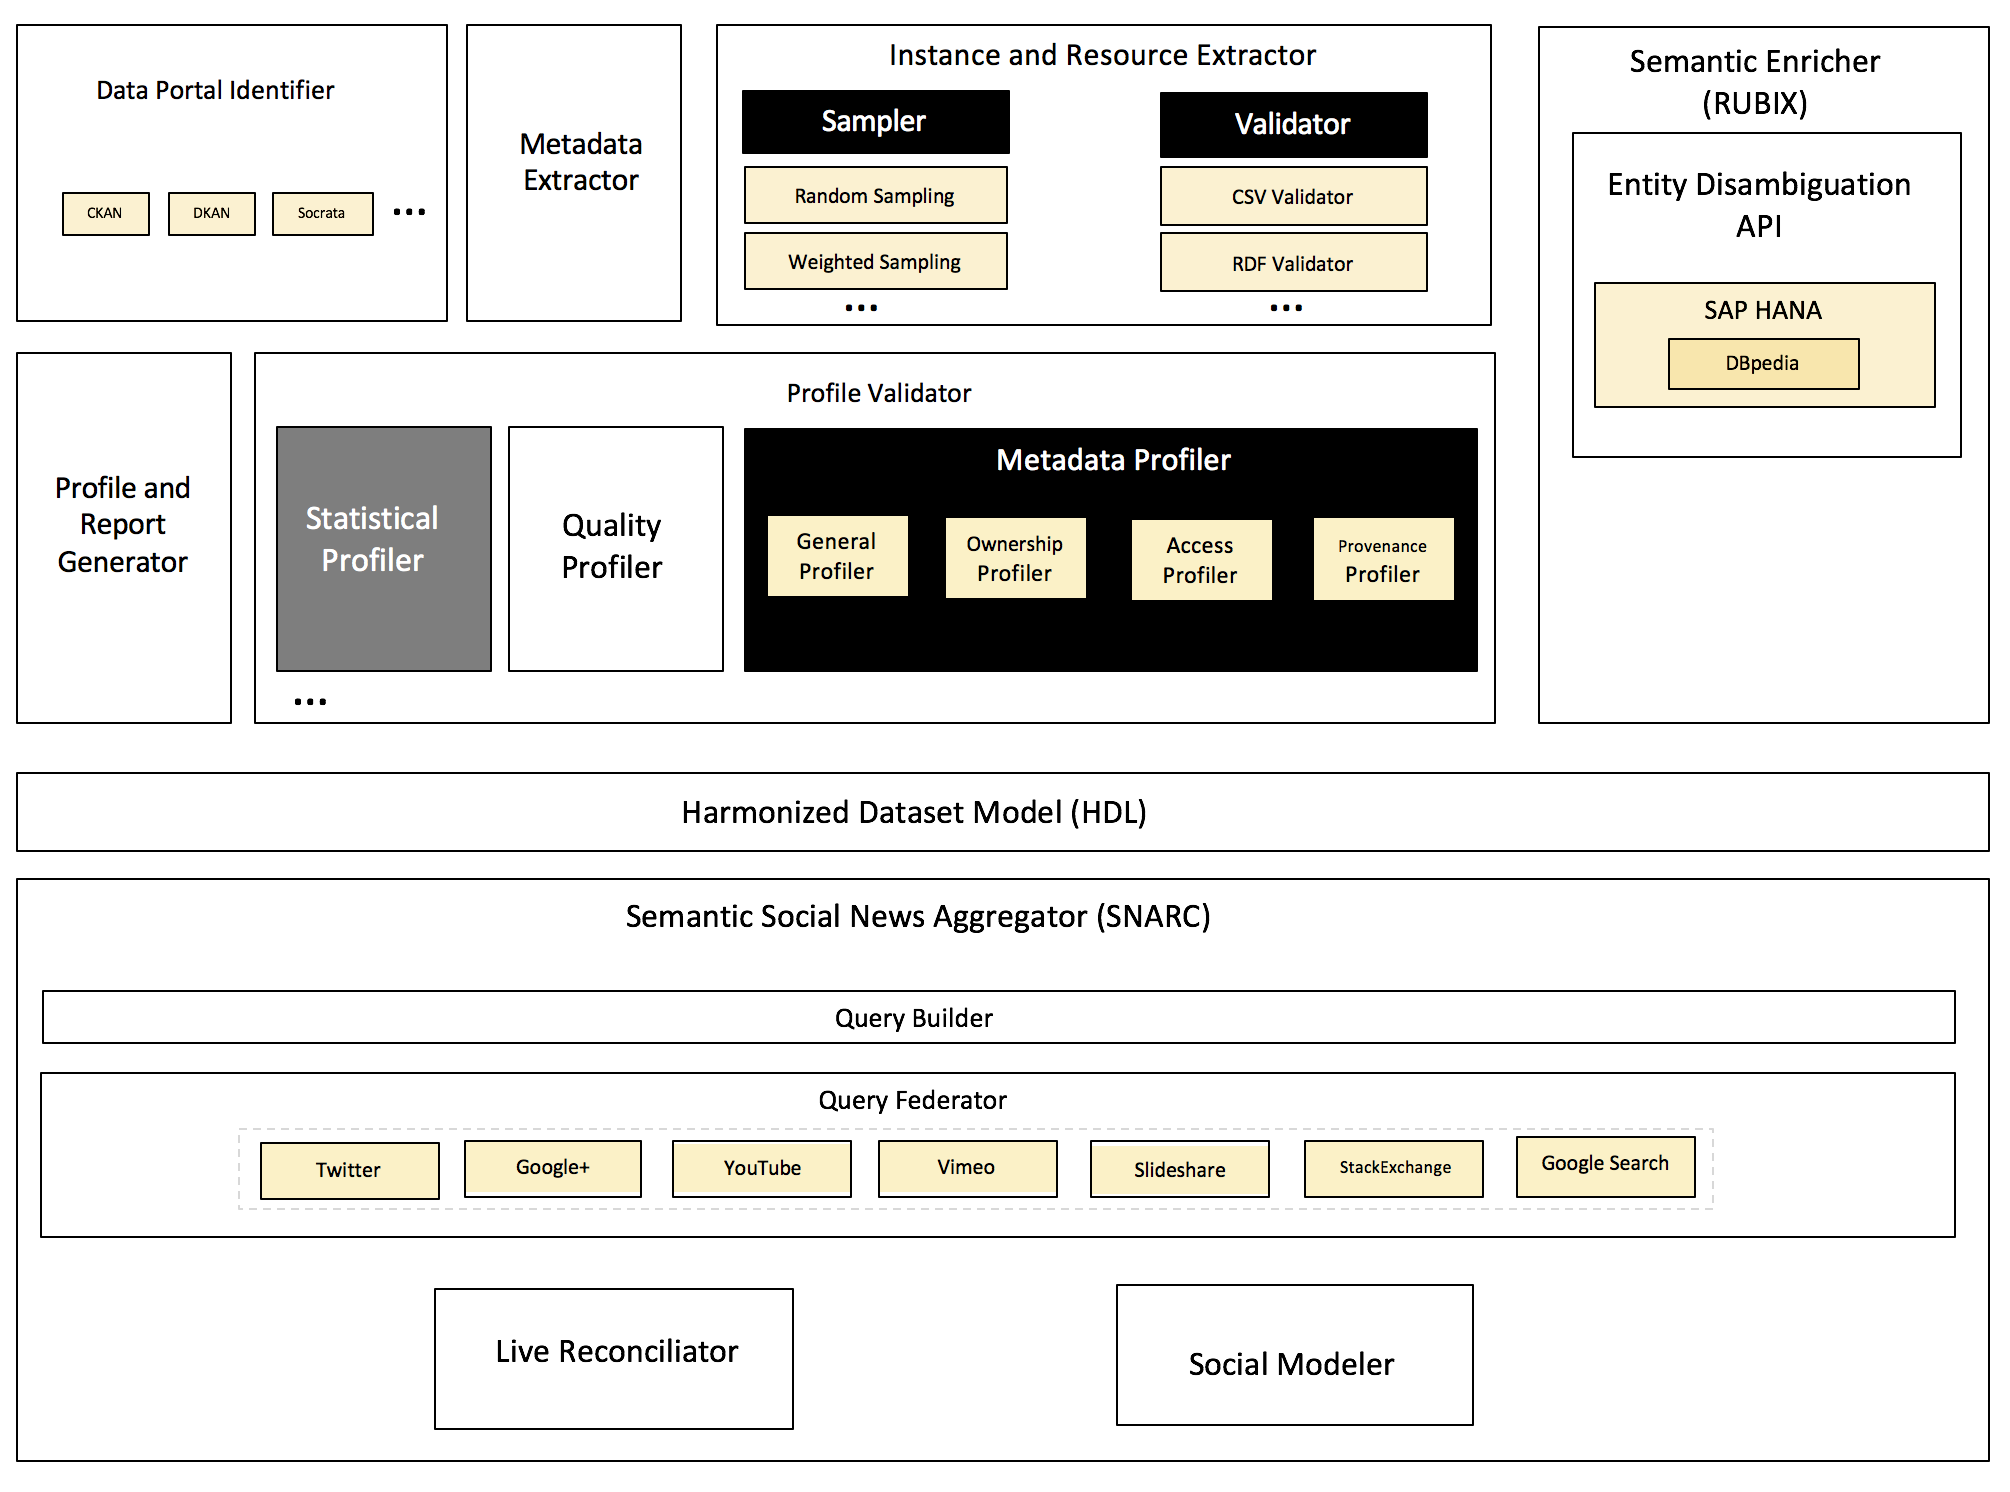
\includegraphics[scale=0.4]{figures/architecutre_diagram.png}
	  \caption{Schéma de l'architecture des données pour permettre l'approvisionnement en libre-service}
	  \label{fig:architecutre_diagram}
	\end{figure}
\end{adjustwidth}

\subsection{Contributions sur Maintenance et Découverte de Données}

En ce qui concerne cet aspect de notre recherche, nous avons accompli les tâches suivantes:
\begin{itemize}
	\item Nous avons interrogé le paysage de différents modèles et des vocabulaires qui décrivent des ensembles de données sur le web. Depuis la création d'un vocabulaire commun ou le modèle est la clé de la communication, nous avons identifié le besoin d'un modèle de métadonnées de jeu de données harmonisée contenant suffisamment d'informations afin que les consommateurs peuvent facilement comprendre et ensembles de données de processus. Premièrement, nous avons mis en place un ensemble de correspondances entre chacune des propriétés des modèles étudiés. Ceci a conduit à la conception de HDL, un modèle de données harmonisée, qui prend le meilleur sur ces modèles et les étend à assurer une couverture complète de métadonnées pour permettre la découverte de données, l'exploration et la réutilisation.
	\item Nous avons analysé le paysage des outils de profilage des ensembles de données et découvert diverses lacunes. En conséquence, nous avons proposé Roomba, un cadre évolutif pour extraire automatique, la validation, la création et de générer des profils d'ensembles de données liées descriptives. Roomba applique plusieurs techniques afin de vérifier la validité des métadonnées fournies et pour générer des informations descriptives et statistiques pour un ensemble de données particulier ou pour un portail de données entière.
\end{itemize}

\subsection{Contributions sur la Qualité de Données}
Concernant nos contributions sur l'évaluation de la qualité Linked Data, nous avons accompli les tâches suivantes:
\begin{itemize}
	\item Nous avons proposé un cadre d'évaluation de la qualité des données liées concentrant sur les mesures objectives des données. Nous avons identifié un total de 64 indicateurs de qualité qui ont été mappés lorsque approprié pour quatre catégories principales (entité, DataSet liens, modèles) correspondant aux principes de la publication de données de base lié.
	\item Sur l'arpentage du paysage des outils de qualité de données, nous avons remarqué un manque dans les outils automatiques pour vérifier les paramètres de qualité de l'ensemble de données proposées dans notre cadre. En conséquence, nous avons étendu Roomba pour effectuer une série de contrôles de qualité des données sur les ensembles de données liés. Notre extension couvre la plupart des indicateurs de qualité proposés avec un accent sur l'exhaustivité, l'exactitude, la provenance et les licences.
\end{itemize}

\subsection{Contributions sur l'intégration et l'enrichissement de Données}

En ce qui concerne cet aspect de notre recherche, nous avons accompli les tâches suivantes:
\begin{itemize}
	\item Nous avons créé un cadre appelé RUBIX qui permet de données d'entreprise potentiellement bruyants brassage-up et des données externes. Le cadre exploite des bases de connaissances de référence pour annoter des données avec un ensemble de concepts sémantiques (métadonnées). Un des avantages de ces métadonnées est d'améliorer le processus d'appariement des sources de données hétérogènes au sein d'une entreprise.
	\item Les métadonnées attachée par RUBIX peut encore être utilisé pour enrichir les ensembles de données existants. Toutefois, les concepts sont souvent représentés avec un grand ensemble de propriétés. Pour mieux recommander le haut ``importants'' propriétés d'un concept, nous inversés ingénieur les choix faits par Google lors de la création des panneaux de graphes de connaissances et présentés ces choix en utilisant explicitement le vocabulaire de Fresnel, de sorte que toute application peut lire ce fichier de configuration pour décider qui propriétés d'une entité qui est intéressant à enrichir.
	\item Agrégation nouvelles sociale pertinente est pas une tâche facile. Nous fournissons une Application Programming Interface (API) qui permet l'agrégation de nouvelles sociale sémantique appelé SNARC. Nous avons conçu un exemple d'application frontend tirant parti des capacités de SNARK pour permettre aux utilisateurs de découvrir instantanément les nouvelles sociale pertinente.
\end{itemize}

%%%%%%%%%%%%%%%%%%%%%%%%%
%%%  Towards A Complete Dataset Profile  %%%
%%%%%%%%%%%%%%%%%%%%%%%%%
\let\cleardoublepage\clearpage\let\cleardoublepage\clearpage
\chapter{Vers un jeu de données complet Profil}\label{chapter:1}

%%%%%%%%%%%%%%%%%%%%%%%%%
%%%  Dataset Profiles and Models  %%%
%%%%%%%%%%%%%%%%%%%%%%%%%

\section{Profils des ensembles de données et modèles}\label{chapter:hdl}

La valeur de l'Open Data est reconnu quand il est utilisé. Pour veiller à ce que, les éditeurs ont besoin pour permettre aux gens de trouver des ensembles de données facilement. Portails de données sont spécifiquement conçus à cet effet. Ils le rendent facile pour les individus et les organisations à stocker, publier et découvrir des ensembles de données.

Portails de données (ou des catalogues de données) sont les points d'entrée pour découvrir les jeux de données publiés. Ils sont curated collections d'ensembles de données de métadonnées qui fournissent un ensemble de services de découverte et d'intégration complémentaires.

Portails de données peuvent être public comme \texttt{Datahub.io} et \texttt{publicdata.eu} ou privé comme \texttt{quandl.com} et \texttt{enigma.io}. Portails privés harnais curated manuellement les données provenant de diverses sources et les exposent à des utilisateurs soit librement, soit par le biais de plans payés. De même, dans certains portails de données publiques, les administrateurs examinent manuellement les informations des bases de données, valider, corriger et attachent des informations de métadonnées approprié. Cette information est principalement sous la forme de balises prédéfinies telles que \textit{médias, géographie, sciences de la vie} pour des raisons d'organisation et de clustering.

Il existe plusieurs systèmes de gestion des données (DMS) qui puissance données publiques portails. CKAN\footnote{\url{http://ckan.org}} est le leader open-source la plate-forme de portail de données du monde alimenter des sites Web comme DataHub, les données publiques de l'Europe et des données ouvertes du gouvernement américain. Modelé sur CKAN, DKAN\footnote{\url{http://nucivic.com/dkan/}} est une distribution Drupal autonome qui est utilisé dans différents portails de données publiques ainsi. En plus de ces portails de données de la tradition, il ya un ensemble d'outils qui permettent d'exposer directement les données API RESTful que comme \texttt{thedatatank.com}.

Un modèle de métadonnées de jeu de données doit contenir suffisamment d'informations afin que les consommateurs peuvent facilement comprendre et traiter les données qui est décrit. Après avoir analysé les modèles d'ensembles de données plus importants, nous trouvons que un ensemble de données peut contenir quatre sections principales:
\begin{itemize}
  \item \textbf{Resources}: Les données brutes réel qui peut être téléchargé ou accessible directement via paramètres IQueryable. Ressources peuvent venir dans différents formats tels que JSON, XML ou RDF.
  \item \textbf{Mots clés}: Connaissance descriptive sur le contenu du jeu de données et de la structure. Cela peut aller de la représentation textuelle simple de termes contrôlés sémantiquement riches. Les tags sont à la base de données définit la recherche et de la découverte.
  \item \textbf{Groups}: Groupes agissent comme des unités organisationnelles qui partagent une sémantique commune. Ils peuvent être considérées comme un groupe ou d'une curation d'ensembles de données basés sur des catégories ou des thèmes communs.
  \item \textbf{Organizations}: Les organisations sont une autre façon d'organiser les ensembles de données. Cependant, ils diffèrent des groupes comme ils ne sont pas construits par la sémantique ou propriétés partagées, mais uniquement sur l'association de l'ensemble de données à un parti d'administration spécifique.
\end{itemize}

Après un examen attentif des différents modèles de données, nous avons regroupé les informations de métadonnées en huit types principaux. Chaque section décrite ci-dessus doit contenir une ou plusieurs de ces types. Par exemple, des ressources ont générale, l'accès, la propriété et la provenance des informations alors que les étiquettes ont des informations générales et de la provenance seulement. Les types d'information sont huit:
\begin{itemize}
 \item \textbf{General information}: The core information about the dataset (e.g., title, description, ID). The most common vocabulary used to describe this information is Dublin Core\footnote{\url{http://dublincore.org/documents/dcmi-terms/}}.
 \item \textbf{Access information}: Information about dataset access and usage (e.g., URL, license title and license URL). In addition to the properties in the models discussed above, there are several vocabularies designed specially to describe data access rights, e.g., Linked Data Rights\footnote{\url{http://oeg-dev.dia.fi.upm.es/licensius/static/ldr/}}, the Open Digital Rights Language (ODRL)\footnote{\url{http://www.w3.org/ns/odrl/2/}}.
 \item \textbf{Ownership information}: Authoritative information about the dataset (e.g., author, maintainer and organization). The common vocabularies used to expose ownership information are Friend-of-Friend (FOAF)\footnote{\url{http://xmlns.com/foaf/spec/}} for people and relationships, vCard~\cite{Iannella:W3C:14} for people and organizations and the Organization ontology~\cite{Reynolds:W3C:14} designed specifically to describe organizational structures.
 \item \textbf{Provenance information}: Temporal and historical information about the dataset creation and update records, in addition to versioning information (e.g., creation data, metadata update data, latest version). Provenance information coverage varies across the modeled surveyed. However, its great importance lead to the development of various special vocabularies like the Open Provenance Model\footnote{\url{http://open-biomed.sourceforge.net/opmv/}} and PROV-O~\cite{Lebo:W3C:13}. DataID~\cite{Brummer::ICSS:14} is an effort to provide semantically rich metadata with focus on providing detailed provenance, license and access information.
 \item \textbf{Geospatial information}: Information reflecting the geographical coverage of the dataset represented with coordinates or geometry polygons. There are several additional models and extensions specifically designed to express geographical information. The Infrastructure for Spatial Information in the European Community (INSPIRE) directive\footnote{\url{http://inspire.ec.europa.eu/}} aims at establishing an infrastructure for spatial information. Mappings have been made between DCAT-AP and the INSPIRE metadata. CKAN provides as well a spatial extension\footnote{\url{https://github.com/ckan/ckanext-spatial}} to add geospatial capabilities. It allows importing geospatial metadata from other resources and supports various standards (e.g., ISO 19139) and formats (e.g., GeoJSON).
 \item \textbf{Temporal information}: Information reflecting the temporal coverage of the dataset (e.g., from date to date). There has been some notable work on extending CKAN to include temporal information. \texttt{govdata.de} is an Open Data portal in Germany that extends the CKAN data model to include information like \texttt{temporal\_granularity}, \texttt{temporal\_coverage\_to} and \\\texttt{temporal\_granularity\_from}.
 \item \textbf{Statistical information}: Statistical information about the data types and patterns in datasets (e.g., properties distribution, number of entities and RDF triples). This information is particularly useful to explore a dataset as it gives detailed insights about the raw data when provided properly. VoID is the only model that provides statistical information about a dataset. VoID defines properties to express different statistical characteristics of datasets like the total number of triples, total number of entities, total number of distinct classes, etc. However, there are other vocabularies such as SCOVO~\cite{Hausenblas:ESWC:09} that can model and publish statistical data about datasets.
 \item \textbf{Quality information}: Information that indicates the quality of the dataset on the metadata and instance levels. In addition to that, a dataset should include an openness score that measures its alignment with the Linked Data publishing standards~\cite{Berners-Lee:W3C:06}. Quality information is only expressed in the POD metadata. However, \texttt{govdata.de} extends the CKAN model also to include a \texttt{ratings\_average} field. Moreover, there are various other vocabularies like daQ~\cite{Debattista:WWW:14} that can be used to express datasets quality. The RDF Review Vocabulary\footnote{\url{http://vocab.org/review/}} can also be used to express reviews and ratings about the dataset or its resources.
\end{itemize}

Since establishing a common vocabulary or model is the key to communication, we identified the need for an harmonized dataset metadata model containing sufficient information so that consumers can easily understand and process datasets. To create the mappings between the different models, we performed various steps:
\begin{itemize}
  \item Examine all the models and vocabularies specifications and documentations.
  \item Examine existing datasets using these models and vocabularies. Data Portals\footnote{\url{http://dataportals.org}} provides a comprehensive list of Open Data Portals from around the world. It was our entry point to find out portals using CKAN or DKAN as their underlying DMS. We also investigated portals known to be using specific DMS. Socrata, for example, maintains a list of Open Data portals using their software on their homepage such as \url{http://pencolorado.org} and \url{http://data.maryland.gov}.
  \item Examine the source code of some portals. This was specifically the case for Socrata as their API returns the raw data serialized as JSON rather than the dataset's metadata. As a consequence, we had to investigate the Socrata Open Data API (SODA) source code\footnote{\url{https://github.com/socrata/soda-java/tree/master/src/main/java/com/socrata/model}} and check the different classes and interfaces.
\end{itemize}

From our survey, we found that a proper integration of Open Data into businesses requires datasets to include the following information:
\begin{itemize}
	\item \textbf{Access information}: a dataset is useless if it does not contain accessible data dumps or query-able endpoints;
	\item \textbf{License information}: businesses are always concerned with the legal implications of using external content. As a result, datasets should include both machine and human readable license information that indicates permissions, copyrights and attributions;
	\item \textbf{Provenance information}: depending on the dataset license, the data might not be legally usable if there are no information describing its authoritative and versioning information. Current models under-specify these aspects limiting the usability of many datasets.
\end{itemize}

Since establishing a common vocabulary or model is the key to communication, we identified the need for a harmonized dataset metadata model containing sufficient information so that consumers can easily understand and process datasets. We have identified four main sections that should be included in the model: resources, groups, tags and organizations. Furthermore, we have classified the information to be included into eight types. Our main contribution is a set of mappings between each properties of those models. This has lead to the design of HDL, a harmonized dataset model, that takes the best out of these models to ensure complete metadata coverage to enable data discovery, exploration and reuse.

%%%%%%%%%%%%%%%%%%%%%%%%%
%%%  Dataset Profiles Generation and Validation  %%%
%%%%%%%%%%%%%%%%%%%%%%%%%
\section{Profils Dataset génération et validation}\label{chapter:roomba}

La nature hétérogène des sources de données reflète directement sur la qualité des données, car ils contiennent souvent incohérentes ainsi que des informations de métadonnées mal interprété et incomplète. En outre, la variation significative de la taille, de formats et la fraîcheur des données, il est plus difficile de trouver des ensembles de données utiles sans connaissance préalable. Cela peut être clairement remarqué dans le LOD Cloud où quelques ensembles de données tels que DBPedia~\cite{Bizer: WebSemJorunal: 09}, Freebase~\cite{Bollacker: SIGMOD: 08} et YAGO~\cite{Suchanek de la WWW: 07} sont favorisés par rapport aux ensembles de données moins populaires qui peuvent inclure des connaissances de domaine spécifique plus adapté pour les tâches à accomplir. Par exemple, pour la tâche de construire des systèmes de recommandation conscients du contexte dans une bibliothèque numérique universitaire sur le nuage LOD, les ensembles de données populaires comme le Web sémantique Dog Food \ footnote {\ url {http://datahub.io/dataset/semantic-web -Dog-alimentaire}}, DBLP \footnote{\url{http://datahub.io/dataset/dblp}} ou Yovisto \footnote{\url{http://datahub.io/dataset/yovisto}} peut être favorisée par rapport à des ensembles de données moins connues, mais plus spécifiques comme VIAF \footnote{\urlhttp://datahub.io/dataset/viaf}} qui relie les fichiers d'autorité de 20 bibliothèques nationales, la liste des vedettes-matière pour les bibliothèques publiques en Espagne \footnote{\url{http://datahub.io/dataset/lista-encabezamientos-materia}} ou les Français recherche de thèse moteur \footnote{\url{http://datahub.io/dataset/thesesfr}}.

Aux utilisateurs d'explorer des ensembles de données dans des portails de données reposant sur les informations de métadonnées fixé par le propriétaire de l'ensemble de données ou l'administrateur du portail de données. Cette information est principalement sous forme de balises prédéfinies telles que \ textit {médias, géographie, sciences de la vie} qui sont utilisés à des fins d'organisation et de clustering. Cependant, la diversité croissante de ces ensembles de données rend plus difficile de les classer dans un nombre fixe de balises qui sont subjectivement attribué sans capturer l'essence et la largeur de l'ensemble de données ~ \ cite {Lalithsena: WI: 13}. En outre, l'augmentation du nombre d'ensembles de données disponibles rend l'examen manuel et la conservation des métadonnées insoutenable même quand confiée à des communautés.

Roomba est un outil que nous construisons pour relever les défis de la validation automatique et génération de profils de jeux de données descriptives. Il est un cadre extensible constitué d'un pipeline de traitement qui combine les techniques d'identification des portails de données, jeux de données rampants et un ensemble de modules enfichables combinant plusieurs tâches de profilage. Le cadre de valider les métadonnées données fournies contre une norme agrégées ensemble d'informations. Champs de métadonnées sont automatiquement corrigées, si possible (par exemple, ajout d'une licence référence URL manquant). En outre, un rapport décrivant toutes les questions qui ne peuvent être résolus automatiquement est créé pour être envoyé par courriel à la responsable de l'ensemble de données. Il existe différents outils de profilage statistiques et d'actualité pour les données relationnelle et Linked. L'architecture du cadre permet d'ajouter facilement les tâches que de profilage supplémentaires. Cependant, dans cette section, nous nous concentrons sur la tâche de métadonnées de jeu de données de profilage, en ignorant les tâches de profilage statistique et d'actualité. Nous validons notre cadre d'un ensemble de profils créés manuellement et vérifier manuellement la précision en examinant les résultats de l'exécution sur diverses données portails de CKAN.

Roomba is built as a Command Line Interface (CLI) application using Node.js and is available on the tools Github repository\footnote{\url{https://github.com/ahmadassaf/opendata-checker/tree/master/test}}. Roomba allows data portal administrators like Roomba est construit comme une application interface de ligne de commande (CLI) en utilisant Node.js et est disponible sur les outils Github référentiel \footnote{\url{https://github.com/ahmadassaf/opendata-checker/tree/master/test}}. Roomba permet aux administrateurs de portail de données comme\textbf{Dan} à:

\begin{itemize}
	\item Fetch informations sur le système de gestion des données de portail
	\item Fetch toutes les informations sur les ensembles de données à partir d'un portail de données
	\item Fetch toutes les informations à partir d'un portail de données de groupes
	\item Crawl, chercher et ensembles de données de cache (un ensemble de données spécifiques, des ensembles de données dans un groupe spécifique, des ensembles de données dans l'ensemble du portail)
	\item Exécuter rapport de l'agrégation sur un groupe spécifique ou sur le portail de données entière
	\item profil un ensemble de données spécifique, un ensemble du groupe ou le portail de données entière
\end{itemize}

Figure \ref{fig:architecutre_diagram} montre les principales étapes sont les suivantes:

\begin{itemize}
	\item \textbf{Identification de système de gestion de données}: Le Portail de données identifiant repose sur plusieurs techniques de grattage Web dans le processus d'identification qui comprend une combinaison de l'inspection de l'URL, meta tags inspection et Document Object Model (DOM) inspection.
	\item \textbf{Extraction de métadonnées}: Après avoir identifié le logiciel de portail sous-jacent, les métadonnées Extractor effectue des requêtes itératives à l'API afin d'aller chercher des ensembles de données de métadonnées et de persister dans un système de cache à base de fichiers. Selon le logiciel de portail, les métadonnées Extractor peut émettre des emplois spécifiques d'extraction. Par exemple, dans les portails basés KAN C, les métadonnées Extractor est capable de ramper et extraire les métadonnées d'un ensemble de données spécifique, tous les ensembles de données dans un groupe spécifique (par exemple, LOD cloud) ou tous les jeux de données du portail.
	\item \textbf{Instance et l'extraction des ressources}: De l'extraction de métadonnées, l'instance et des ressources Extractor est capable d'identifier toutes les ressources associées à ce jeu de données. Ils peuvent avoir différents types comme un critère SPARQL, API, fichier, visualisation, etc. Cependant, avant d'extraire l'instance (s) de ressource. Considérant que certains ensembles de données contiennent de grandes quantités de ressources et de la puissance de calcul limitée de certaines machines sur lesquelles le cadre pourrait fonctionner sur un sous-module Sampler est introduit pour exécuter différentes stratégies à base d'échantillons comme ils ont été trouvés pour produire des résultats précis, même avec petit échantillon comparable taille de 10\%~\cite{Fetahu:ESWC:14}.
	\item \textbf{validation Profil}: Le Profil Validator (composant (iv)) identifie les informations manquantes et la capacité de les corriger automatiquement. Chaque ensemble de métadonnées (général, l'accès, la propriété et la provenance) est validée et corrigée automatiquement lorsque possible. Chaque tâche de profileur a un ensemble de champs de métadonnées pour vérifier contre. Le processus de validation vérifier si chaque champ est défini et si la valeur attribuée est valide.

	Il existe de nombreuses mesures spéciales de validation pour divers domaines. Par exemple, les adresses électroniques et les URL doivent être validés pour garantir que la valeur entrée est syntaxiquement correct. En plus de cela, pour les URL, le Profil Validator émet un HTTP \texttt{HEAD} demande afin de vérifier si cette URL est accessible. Le Profil Validator utilise également les informations contenues dans un \texttt{content-tête} réponse valide à extraire, comparer et corriger certaines valeurs de métadonnées des ressources comme \texttt{mimetype} et \texttt{size}.
	\item \textbf{Profil et la génération de rapports}: Tprocessus de validation, il met en évidence les informations manquantes et les présente dans un rapport lisible par l'homme. Le rapport peut être automatiquement envoyé à l'email de données mainteneur si elle existe dans les métadonnées. En plus du rapport généré, les profils améliorés sont représentés dans JSON en utilisant le modèle de données de CKAN et sont accessibles au public \footnote{\url{https://github.com/ahmadassaf/opendata-checker/tree/master/results}}.
\end{itemize}

Nous avons couru notre outil sur deux portails de données basés sur CKAN. Le premier est le DataHub ciblant spécifiquement le groupe des nuages ​​LOD. L'état actuel du rapport de cloud LOD~\cite{Schmachtenberg: ISWC: 14} indique que le LOD nuage contient 1014 jeux de données. Ils ont été récoltées via un robot de LDSpider~\cite{Isele: ISWC: 10} ensemencé avec 560 milliers URI. Roomba d'autre part, récupère les ensembles de données hébergées dans les portails de données où les ensembles de données ont attachés métadonnées pertinentes. En conséquence, nous nous sommes appuyés sur les informations fournies par l'API DataHub CKAN. Examiner les balises disponibles, nous avons trouvé deux groupes de candidats. La première marqués avec ``lodcloud'' returned 259 ensembles de données, tandis que le second marqués avec ``lod'' retourné seulement 75 ensembles de données. Après avoir examiné manuellement les deux listes, nous avons découvert les jeux de données groupées avec la balise ``lodcloud'' sont les bons car ils contenaient des métadonnées plus récente et précise. Pour se qualifier d'autres portails CKAN-pour les expériences, nous avons utilisé \texttt{dataportals.org}, qui contient une liste complète des portails Open Data à travers le monde. Nous avons choisi d'Amsterdam portail de données\footnote{\url{http://data.amsterdamopendata.nl/}} comme il est mis à jour fréquemment et fortement maintenue. Le portail a été commandée en 2012 par le Conseil économique ouvert d'échange de données d'Amsterdam (ODE), et couvre un large éventail de domaines d'information (énergie, économie, l'éducation, le développement urbain, etc.) sur Amsterdam région métropolitaine.

Dans notre évaluation, nous nous sommes concentrés sur deux aspects: i) \textit{exactitude profilage} qui évalue manuellement la validité des erreurs générées dans le rapport, et ii) \textit{exhaustivité profilage} qui évalue si les profileurs couvrent toutes les erreurs les métadonnées des ensembles de données.

Notre évaluation a montré que le Roomba a exactitude et l'exhaustivité complète pour les propriétés examinées. En conséquence, nous avons couru Roomba sur le groupe de nuages ​​LOD hébergé dans le DataHub. Nous avons découvert que l'état général de l'ensemble des données examinées a besoin d'attention, car la plupart d'entre eux manquent d'informations d'accès informatif et leurs ressources souffrent faible disponibilité. Ces deux mesures sont d'une grande importance pour les entreprises qui cherchent à intégrer et utiliser des données externes dont le lien. Nous avons découvert que l'information la plus erronée de l'information de base de données sont la propriété liée puisque cette information est manquante ou undefined pour 41\% des ensembles de données. Ressources jeux de données ont les métadonnées les plus pauvres: 64\% des métadonnées générale, toutes les informations d'accès et 80\% de l'information contenue sur la provenance des valeurs manquantes ou non définis. Nous avons également montré que le processus de correction automatique peut effectivement améliorer la qualité de certaines informations. Nous croyons qu'il ya un besoin d'avoir un effort communautaire pour corriger manuellement manque des informations importantes comme des informations de propriété (mainteneur, auteur et mainteneur et auteur e-mails).

\section{Objective Linked Data Quality Assessment}\label{chapter:data-quality}

We are entering an era where open is the new default. Governments, universities, organizations and even individuals are publicly publishing huge amounts of open data. This openness should be accompanied with a certain level of trust or guarantees about the quality of data. The Linked Open Data is a gold mine for those trying to leverage external data sources in order to produce more informed business decisions~\cite{Boyd:Article:11}. However, the heterogeneous nature of sources reflects directly on the data quality as these sources often contain inconsistent as well as misinterpreted and incomplete information.

Traditional data quality is a thoroughly researched field with several benchmarks and frameworks to grasp its dimensions~\cite{Kahn:ACM:02,Stvilia:ASIST:07,Wang:MIS:96}. Data quality principles typically rely on many subjective indicators that are complex to measure automatically. The quality of data in indeed realized when it is used~\cite{Juran:McGraw:99}, thus directly relating to the ability of satisfying users' continuous needs.

Web documents that are by nature unstructured and interlinked require different quality metrics and assessment techniques than traditional datasets. For example, the importance and quality of Web documents can be subjectively calculated via algorithms like Page Rank~\cite{ Page:TechReport:98}. Despite the fact that Linked Open Data quality is a trending and highly demanded topic, very few efforts are currently trying to standardize, track and formalize frameworks to issue scores or certificates that will help data consumers in their integration tasks.

Data quality assessment is the process of evaluating if a piece of data meets the consumers need in a specific use case~\cite{Bizer:WebSemantics:09}. The dimensionality of data quality makes it dependent on the task and users requirements. For example, DBpedia~\cite{Bizer:WebSemJorunal:09} and YAGO~\cite{Suchanek::WWW:07} are knowledge bases containing data extracted from structured and semi-structured sources. They are used in a variety of applications  e.g., annotation systems~\cite{Mendes:ICS:11}, exploratory search~\cite{Marie:ICS:13} and recommendation engines~\cite{DiNoia:iSemantics:12}. However, their data is not integrated into critical systems e.g., life critical (e.g., medical applications) or safety critical (e.g., aviation applications) as its data quality is found to be insufficient.

The basic idea behind Linked Data is that its usefulness increases when it is more interlinked with other datasets. Tim Berners-Lee defined four main principles for publishing data that can ensure a certain level of uniformity reflecting directly data's usability~\cite{Berners-Lee:W3C:06}:

\begin{itemize}
	\item \textbf{Make the data available on the Web}: assign URIs to identify things.
	\item \textbf{Make the data machine readable}: use HTTP URIs so that looking up these names is easy.
	\item \textbf{Use publishing standards}: when the lookup is done provide useful information using standards like RDF.
	\item \textbf{Link your data}: include links to other resources to enable users to discover more things.
\end{itemize}

\noindent
Building on these principles, we group the quality attributes into four main categories:

\begin{itemize}
	\item \textbf{Quality of the entities }: quality indicators that focus on the data at the instance level.
	\item \textbf{Quality of the dataset}: quality indicators at the dataset level.
	\item \textbf{Quality of the semantic model}: quality indicators that focus on the semantic models, vocabularies and ontologies.
	\item \textbf{Quality of the linking process}: quality indicators that focus on the inbound and outbound links between datasets.
\end{itemize}

In~\cite{Assaf:DQMST:12}, the authors identified 24 different Linked Data quality attributes. These attributes are a mix of objective and subjective measures that may not be derived automatically. In this paper, we refine these attributes into a condensed framework of 10 objective measures. Since these measures are rather abstract, we should rely on quality indicators that reflect data quality~\cite{Flemming:Thesis:10} and use them to automate calculating datasets quality.

The quality indicators are weighted. These weights give the flexibility to define multiple degrees of importance. For example, a dataset containing people can have more than one person with the same name thus it is not always true that two entities in a dataset should not have the same preferred label. As a result, the weight for that quality indicator will be set to zero and will not affect the overall quality score for the consistency measure.

Independent indicators for entity quality are mainly subjective e.g., the degree to which all the real-world objects are represented, the scope and level of details, etc. However, since entities are governed by the underlying model, we have grouped their indicators with those of the modeling quality.

Table~\ref{DQM} lists the refined measures alongside their objective quality indicators. Those indicators have been gathered by:

\begin{itemize}
	\item Transforming the objective quality indicators presented as a set of questions in~\cite{Assaf:DQMST:12} into more concrete quality indicator metrics.
	\item Surveying the landscape of data quality tools and frameworks.
	\item Examining the properties of the most prominent linked data models from the survey done in~\cite{Assaf:PROFILES:15}.
\end{itemize}


\begin{center}
{\footnotesize
\setlength\LTleft{-.5in}
\setlength\LTright{-.5in}
\begin{longtable}[h]{|c|c|c|l|}
\caption[Objective Linked Data quality framework]{Objective Linked Data quality framework} \label{DQM} \\

\hline \multicolumn{1}{|c|}{\textbf{Quality Attribute}} & \multicolumn{1}{c|}{\textbf{Quality Category}} & \multicolumn{1}{c|}{\textbf{ID}} & \multicolumn{1}{c|}{\textbf{Quality Indicator}} \\ \hline
\endfirsthead

\multicolumn{4}{c}%
{{\bfseries \tablename\ \thetable{} Objective Linked Data quality framework}} \\
\hline \multicolumn{1}{|c|}{\textbf{Quality Attribute}} &
\multicolumn{1}{c|}{\textbf{Quality Category}} & \textbf{ID} &
\multicolumn{1}{c|}{\textbf{Quality Indicator}} \\ \hline
\endhead

\multicolumn{4}{|r|}{{Continued on next page}} \\ \hline
\endfoot

\endlastfoot

\multirow{15}{*}{Completeness}
 & \multirow{5}{*}{Dataset Level} & 1 & Existence of supporting structured metadata ~\cite{Hogan:LDOW:10}\tabularnewline
\cline{3-4}
 &  & 2 & Supports multiple serializations~\cite{Zaveri:SemWebJorunal:12}\tabularnewline
\cline{3-4}
 &  & 3 & Has different data access points \tabularnewline
\cline{3-4}
 &  & 4 & Uses datasets description vocabularies \tabularnewline
\cline{3-4}
 &  & 5 & Existence of descriptions about its size \tabularnewline
 \cline{3-4}
 &  & 6 & Existence of descriptions about its structure (MIME Type, Format) \tabularnewline
 \cline{3-4}
 &  & 7 & Existence of descriptions about its organization and categorization \tabularnewline
 \cline{3-4}
 &  & 8 & Existence of information about the kind and number of used vocabularies~\cite{Zaveri:SemWebJorunal:12}\tabularnewline
\cline{2-4}
 & \multirow{1}{*}{Links Level} & 9 & Existence of dereferencable links for the dataset~\cite{Hogan:LDOW:10,Mader:TBDL:12,Gueret:ESWC:12}\tabularnewline \hline
\cline{2-4}
 & \multirow{4}{*}{Model Level} & 10 & Absence of disconnected graph clusters~\cite{Mader:TBDL:12}\tabularnewline
\cline{3-4}
 &  & 11 & Absence of omitted top concept~\cite{Hogan:LDOW:10}\tabularnewline
 \cline{3-4}
 &  & 12 & Has complete language coverage~\cite{Mader:TBDL:12}\tabularnewline
\cline{3-4}
 &  & 13 & Absence of unidirectional related concepts~\cite{Hogan:LDOW:10}\tabularnewline
 \cline{3-4}
 &  & 14 & Absence of missing labels~\cite{Mader:TBDL:12}\tabularnewline
 \cline{3-4}
 &  & 15 & Absence of missing equivalent properties~\cite{Maria:KEOD:13}\tabularnewline
 \cline{3-4}
 &  & 16 & Absence of missing inverse relationships~\cite{Maria:KEOD:13}\tabularnewline
 \cline{3-4}
 &  & 17 & Absence of missing domain or range values in properties~\cite{Maria:KEOD:13}\tabularnewline
\hline
\hline
\multirow{2}{*}{Availability} & \multirow{2}{*}{Dataset Level} & 18 & Existence of an RDF dump that can be downloaded by users~\cite{Flemming:Thesis:10}\cite{Hogan:LDOW:10}\tabularnewline
\cline{3-4}
 &  & 19 & Existence of a queryable endpoint that responds to direct queries \tabularnewline
\cline{3-4}
 &  & 20 & Existence of valid dereferencable URLs (respond to HTTP request) \tabularnewline
\hline
\hline
\multirow{3}{*}{Licensing} & \multirow{3}{*}{Dataset Level} & 21 & Existence of human and machine readable license information~\cite{Hogan:WebSemJorunal:12}\tabularnewline
\cline{3-4}
 &  & 22 & Existence of de-referenceable links to the full license information~\cite{Hogan:WebSemJorunal:12}\tabularnewline
\cline{3-4}
 &  & 23 & Specifies permissions, copyrights and attributions~\cite{Zaveri:SemWebJorunal:12}\tabularnewline
\hline
\hline
\multirow{1}{*}{Freshness} & \multirow{1}{*}{Dataset Level} & 24 & Existence of timestamps that can keep track of its modifications ~\cite{Flouris:EvoDyn:12}\tabularnewline
\hline
\hline
\multirow{11}{*}{Correctness}  & \multirow{2}{*}{Dataset Level} & 25 & Includes the correct MIME-type for the content ~\cite{Hogan:LDOW:10}\tabularnewline
\cline{3-4}
 &  & 26 & Includes the correct size for the content \tabularnewline
 \cline{3-4}
 &  & 27 & Absence of syntactic errors on the instance level~\cite{Hogan:LDOW:10}\tabularnewline
\cline{2-4}
 & \multirow{2}{*}{Links Level} & 28 & Absence of syntactic errors~\cite{Suominen:DataSemantics:13}\tabularnewline
 \cline{3-4}
 &  & 29 & Use the HTTP URI scheme (avoid using URNs or DOIs)~\cite{Mader:TBDL:12}\tabularnewline
\cline{2-4}
 & \multirow{7}{*}{Model Level} & 30 & Contains marked top concepts~\cite{Mader:TBDL:12}\tabularnewline
\cline{3-4}
 &  & 31 & Absence of broader concepts for top concepts~\cite{Mader:TBDL:12}\tabularnewline
 \cline{3-4}
 & & 32 & Absence of missing or empty labels~\cite{Acosta:ISWC:13,Mader:TBDL:12}\tabularnewline
  \cline{3-4}
 & & 33 & Absence of unprintable characters~\cite{Acosta:ISWC:13,Mader:TBDL:12} or extra white spaces in labels~\cite{Suominen:IKEM:12}\tabularnewline
\cline{3-4}
 &  & 34 & Absence of incorrect data type for typed literals~\cite{Hogan:LDOW:10,Acosta:ISWC:13} \tabularnewline
\cline{3-4}
 &  & 35 & Absence of omitted or invalid languages tags~\cite{Suominen:IKEM:12,Mader:TBDL:12}\tabularnewline
\cline{3-4}
 &  & 36 & Absence of terms without any associative or hierarchical relationships\tabularnewline
\hline
\hline
\multirow{7}{*}{Comprehensibility} & \multirow{4}{*}{Dataset Level} & 37 & Existence of at least one exemplary RDF file~\cite{Zaveri:SemWebJorunal:12}\tabularnewline
\cline{3-4}
 &  & 38 & Existence of at least one exemplary SPARQL query~\cite{Zaveri:SemWebJorunal:12}\tabularnewline
 \cline{3-4}
 &  & 39 &  Existence of general information (title, URL, description) for the dataset \tabularnewline
\cline{3-4}
 &  & 40 & Existence of a mailing list, message board or point of contact~\cite{Flemming:Thesis:10}\tabularnewline
 \cline{2-4}
 & \multirow{3}{*}{Model Level} & 41 & Absence of misuse of ontology annotations~\cite{Mader:TBDL:12,Maria:KEOD:13}\tabularnewline
  \cline{3-4}
 & & 42 & Existence of annotations for concepts~\cite{Maria:KEOD:13}\tabularnewline
 \cline{3-4}
 & & 43 & Existence of documentation for concepts~\cite{Mader:TBDL:12,Maria:KEOD:13}\tabularnewline
\hline
\hline
\multirow{3}{*}{Provenance} & \multirow{2}{*}{Dataset Level} & 44 & Existence of metadata that describes its authoritative information ~\cite{Flouris:EvoDyn:12}\tabularnewline
\cline{3-4}
 &  & 45 & Usage of a provenance vocabulary\tabularnewline
 \cline{3-4}
 &  & 46 & Usage of a versioning\tabularnewline
\hline
\hline
\multirow{10}{*}{Coherence} & \multirow{10}{*}{Model Level} & 47 & Absence of misplaced or deprecated classes or properties ~\cite{Hogan:LDOW:10}\tabularnewline
\cline{3-4}
 &  & 48 & Absence of relation and mappings clashes ~\cite{Suominen:IKEM:12}\tabularnewline
\cline{3-4}
 &  & 49 & Absence of blank nodes~\cite{Hogan:WebSemJorunal:12}\tabularnewline
\cline{3-4}
 &  & 50 & Absence of invalid inverse-functional values~\cite{Hogan:LDOW:10}\tabularnewline
\cline{3-4}
 &  & 51 & Absence of cyclic hierarchical relations~\cite{Dagobert:DL:02,Suominen:IKEM:12,Mader:TBDL:12}\tabularnewline
\cline{3-4}
 &  & 52 & Absence of undefined classes and properties usage~\cite{Hogan:LDOW:10}\tabularnewline
\cline{3-4}
 &  & 53 & Absence of solely transitive related concepts~\cite{Mader:TBDL:12}\tabularnewline
\cline{3-4}
 &  & 54 & Absence of redefinitions of existing vocabularies ~\cite{Hogan:LDOW:10}\tabularnewline
\cline{3-4}
 &  & 55 & Absence of valueless associative relations ~\cite{Mader:TBDL:12}\tabularnewline
\hline
\hline
\multirow{7}{*}{Consistency}
 & \multirow{7}{*}{Model Level}
& 56 & Consistent usage of preferred labels per language tag~\cite{Isaac:W3C:09,Mader:TBDL:12}\tabularnewline
 \cline{3-4}
 & & 57 & Consistent usage of naming criteria for concepts~\cite{Maria:KEOD:13}\tabularnewline
\cline{3-4}
 &  & 58 & Absence of overlapping labels\tabularnewline
\cline{3-4}
 &  & 59 & Absence of disjoint labels~\cite{Mader:TBDL:12}\tabularnewline
\cline{3-4}
 & & 60 & Absence of atypical use of collections, containers and reification~\cite{Hogan:LDOW:10}\tabularnewline
\cline{3-4}
 &  & 61 & Absence of wrong equivalent, symmetric or transitive relationships~\cite{Maria:KEOD:13}\tabularnewline
\cline{3-4}
 &  & 62 & Absence of membership violations for disjoint classes~\cite{Hogan:LDOW:10}\tabularnewline
\hline
\hline
\multirow{2}{*}{Security} & \multirow{2}{*}{Dataset Level} & 63 & Uses login credentials to restrict access~\cite{Zaveri:SemWebJorunal:12}\tabularnewline
\cline{3-4}
 &  & 64 & Uses SSL or SSH to provide access to their dataset~\cite{Zaveri:SemWebJorunal:12}\tabularnewline
\hline
\end{longtable}
}
\end{center}


We have extended Roomba with 7 submodules that will check various dataset quality indicators. Some indicators have to be examined against a finite set. Since Roomba runs on CKAN-based data portals, we built our quality extension to calculate the scores against the CKAN standard model.


A CKAN portal contains a set of datasets $\textbf{D} = \{D_1,...D_n\}$. We denote the set of resources $R_i = \{r_1,...,r_k\}$, groups $G_i = \{g_1,...,g_k\}$ and tags $T_i = \{t_1,...,t_k\}$ for $D_i \in \textbf{D} (i=1,...,n)$ by $  \textbf{R}=\{R_1,...,R_n\}, \textbf{G}=\{G_1,...,G_n\}$ and $\textbf{T}=\{T_1,...,t_n\}$ respectively.

Our quality framework contains a set of measures $\textbf{M} = \{M_1,...,M_n\}$. We denote the set of quality indicators $Q_i = \{q_1,...,q_k\}$ for $M_i \in \textbf{M} (i=1,...,n)$ by $\textbf{Q} = \{Q_1,...,Q_n\}$. Each quality indicator has a weight, context and a score $Q_i<weight, context, score>$. In Roomba, all the weights are equal and set to 1. However, they can be adjusted manually to rank the quality indicators. Each $Q_i$ of $M_i$ (for $i$ = 1,...$n$) is applied to one or more of the resources, tags or groups. The indicator context is defined where $\exists Q_i \in \textbf{R} \cup \textbf{G} \cup \textbf{T}$.

The quality indicator score is based on a ratio between the number of violations $\textbf{V}$ and the total number of instances where the rule applies $\textbf{T}$ multiplied by the specified weight for that indicator. In some cases, the quality indicator score is a boolean value (0 or 1). For example, checking if there is a valid metadata file (QI.1) or checking if the \texttt{license\_url} is dereferenceable (QI.22).


\begin{equation}
 Q\textrm{ weightedscore} = (V/T) * Q<weight>
\end{equation}

$Q\textrm{ weightedscore}$ is an error ratio. A quality measure score should reflect the alignment of the dataset with respect to the quality indicators. The quality measure score \textbf{M} is calculated by dividing the weighted quality indicator scores sum by the total number of instances in its context, as the following formula shows:

\begin{equation}
M =  1 - ((\sum_{i=1}^{n} Q\textrm{i weightedscore}) / \mid Qi\textrm{ context} \mid )
\end{equation}

Roomba covers 82\% of the suggested datasets objective quality indicators. Based on our experiments running Roomba on the LOD cloud, we discovered that the general state of the datasets needs attention as most of them have low completeness, provenance, licensing and comprehensibility quality scores.

%%%%%%%%%%%%%%%%%%%%%%%%%
%%%  Towards Enriched Enterprise Data  %%%
%%%%%%%%%%%%%%%%%%%%%%%%%
\let\cleardoublepage\clearpage
\chapter{Vers Enrichi de données d'entreprise}\label{chapter:2}

\section{Intégration des données dans l'entreprise}\label{chapter:rubix}
Les entreprises ont traditionnellement effectué une analyse d'affaires basé sur les données transactionnelles existants stockés dans des bases de données relationnelles. Les données d'entreprise disponibles pour les décideurs était généralement la gestion des relations ou des données de planification des ressources d'entreprise. Cependant médias sociaux nourrit, les weblogs, les données des capteurs, ou des données publiées par les gouvernements ou organisations internationales sont de nos jours de plus en plus disponibles~\cite{Boyd:Article:11}.

La qualité et la quantité de connaissance structurée disponibles rendent désormais possible pour les entreprises de la mienne cette énorme quantité de données publiques et de l'intégrer dans leurs systèmes de gestion d'information d'entreprise de prochaine génération. L'analyse de ce nouveau type de données dans le contexte des données d'entreprise existantes devrait leur apporter de nouvelles ou plus précises des analyses commerciales et permettre une meilleure reconnaissance du chiffre d'affaires et des opportunités de marché~\cite{LaValle:MIT:11}.

Ces nouvelles sources distribuées, cependant, posent des défis énormes. Ils ont fondamentalement différents formats de fichiers, les protocoles d'accès ou des langages de requête. Ils possèdent leur propre modèle de données avec différentes façons de représenter et stocker les données. Données à travers ces sources peuvent être bruyant (par exemple, dupliquer ou incohérentes), incertain ou être sémantiquement similaire pourtant différent. Intégration et la fourniture d'une vue unifiée pour ces structures de données hétérogènes et complexes nécessitent donc des outils puissants pour cartographier et organiser les données.

Établir des bases de connaissances de données dans l'entreprise peut faciliter la fourniture de services d'intégration de données~\cite{Frischmuth:SemWebJorunal:12}. Dans cette section, nous présentons notre travail en utilisant DBpedia comme une base de connaissances interne. Nous présentons en outre un ensemble de services que nous mis en place sur le dessus de DBpedia permettant entité homonymie et l'amélioration de schéma correspondant. Ces services permettent aux utilisateurs d'affaires de combiner semi-automatiquement des données potentiellement bruyants résidant dans des silos hétérogènes. Sémantiquement données connexes est identifié et correspondances appropriées sont proposées aux utilisateurs. En cas d'acceptation de l'utilisateur, les données sont agrégées et peut être visualisé directement ou exporté vers des outils de reporting de Business Intelligence. Enfin, nous procédons à une ingénierie inverse du panneau Google graphique de connaissances pour savoir quelles sont les propriétés les plus pertinents pour une entité. Nous comparons ces résultats avec un sondage, nous avons mené sur 152 utilisateurs et nous montrons comment nous pouvons représenter et explicite cette connaissance en utilisant le vocabulaire de Fresnel.

Schema correspondant est généralement utilisé dans les affaires de l'intégration de l'entreprise, métamodèle correspondant, ainsi que les processus ETL. Pour les non-spécialistes IT la manière typique de comparer les données financières à partir de deux ans ou quartiers différents, par exemple, serait de copier et coller les données d'une feuille de calcul Excel dans un autre, créant ainsi des licenciements et potentiellement introduire des erreurs de copier-coller . En utilisant des techniques d'adaptation de schéma, il est possible de soutenir ce processus semi-automatique, soit pour déterminer les colonnes qui sont similaires et les proposer à l'utilisateur pour l'intégration. Cette intégration peut être fait avec des outils de business intelligence appropriées qui fournissent des visualisations.

Un des problèmes dans l'exécution de l'intégration est la qualité des données. Les colonnes peuvent contenir des données qui est bruyant ou incorrecte. Il peut aussi y avoir aucun têtes de colonne pour fournir des informations appropriées pour la correspondance. Un certain nombre d'approches exploiter les similitudes de têtes ou les similitudes des types de données de colonne. Nous avons proposé une nouvelle approche qui exploite le typage sémantique riche fourni par notre homonymie de l'entité.

\subsection{Rapprochement des données}
Réconciliation permet entité homonymie, à savoir les cellules correspondant à des entités typés correspondant en cas de données tabulaires. Google Préciser prend déjà en charge la réconciliation avec Freebase, mais nécessite une confirmation de l'utilisateur. Pour les moyennes et grandes bases de données, cela peut être très chronophage. Pour réconcilier les données, nous avons donc d'abord identifier les colonnes qui sont candidats à la réconciliation en sautant les colonnes contenant des valeurs ou des dates numériques. Nous utilisons ensuite l'API d'homonymie pour interroger pour chaque cellule des colonnes source et cible de la liste des entités typées candidats. Les résultats sont mis en cache afin d'être récupérés par nos algorithmes de similarité.

\subsection{Colonnes sans nom et non typés correspondant}
L'AMC a la capacité de combiner les résultats de différents algorithmes correspondant. Son défaut intégré correspondant algorithmes travaillent sur-têtes de colonnes et de produire un score global de similitude entre les éléments de schéma rapport. Il a été prouvé que la combinaison de différents algorithmes augmente considérablement la qualité des résultats correspondant~\cite{Peukert:ICDE:12}\cite{conf/wise/StracciaT05}. Toutefois, lorsque les en-têtes sont manquants ou ambiguë, l'AMC ne peut exploiter les algorithmes domaine d'intersection et d'inclusion sur la base de données de la colonne. Nous avons donc mis en place trois nouveaux algorithmes de similarité qui exploitent les types riches extraites de données liées en vue d'améliorer les résultats correspondants de colonnes anonymes ou non typées. Ils sont présentés ci-dessous.

\begin{itemize}
	\item \textbf{Cosine Similarity}: On compare le vecteur de résultat des types de candidats à partir de la colonne de la source avec le vecteur de résultat des types de candidats à partir de la colonne cible. Les similitudes $s$ entre la paire de colonnes peuvent être calculées en utilisant la valeur absolue de la fonction cosinus de similitude.
	\item \textbf{Pearson Product-Moment Correlation Coefficient (PPMCC)}: Le deuxième algorithme qui nous avons implémenté est PPMCC, une mesure statistique de l'indépendance linéaire entre deux variables $\left(x,y\right)$~\cite{Kowalski:RoyalStat:72}. L'entrée pour PPMC se compose de deux tableaux qui représentent les valeurs de la source et de colonnes cibles, où la colonne source est la colonne avec le plus grand ensemble de types riches trouvé.
	\item \textbf{Spearman's Rank Correlation Coefficient}: Le dernier algorithme qui nous avons implémenté pour correspondre colonnes anonymes et non typées est le coefficient de corrélation de rang de Spearman. Il applique une transformation de rang sur les données d'entrée et ordinateur PMCC après sur les données classées. Dans nos expériences, nous avons utilisé Classement naturel avec les stratégies par défaut pour le traitement des liens et les valeurs NaN. L'algorithme de classement est toutefois configurable et peut être améliorée en utilisant des mesures plus sophistiquées.
\end{itemize}

\subsection{colonne étiquetage}

Nous avons montré dans la section précédente comment faire correspondre les colonnes anonymes et non typées. L'étiquetage de la colonne est cependant bénéfique que les résultats de nos algorithmes précédentes peuvent être combinées avec des techniques traditionnelles tête correspondants à améliorer la qualité de l'appariement.

Types riches extraites de Freebase sont indépendantes l'une de l'autre. Nous avons besoin de trouver une méthode qui permettra de déterminer score normalisé pour chaque type dans le jeu en équilibrant la proportion de scores élevés avec celles du bas à l'aide de Wilson marquer intervalle pour un paramètre de Bernoulli.

\subsection{Manipulation non-valeurs de String}

Jusqu'à présent, nous avons couvert plusieurs méthodes pour identifier la similitude entre ``String'' valeurs, mais que diriez-vous d'autres valeurs numériques telles que les dates, l'argent, la distance, etc. A cet effet, nous avons mis en place un certain type identificateur de base qui peut reconnaître dates, argent, valeurs numériques, les chiffres utilisés comme identifiants. Cela nous aidera à mieux entrées match correspondant. Réglage des algorithmes de combinaison de AMC peut être d'une grande importance à ce stade. Par exemple, l'attribution de pondérations à différents adaptateurs et peaufiner la configuration peut donner des résultats plus précis.

\subsection{Propriétés importantes pour les entités}\label{Section:EKG}

Les entités sont généralement décrits avec beaucoup de propriétés. Cependant, toutes les propriétés ont la même importance. Certaines propriétés sont considérés comme clés pour effectuer des tâches d'instance correspondant tandis que d'autres propriétés sont généralement choisis pour fournir rapidement un résumé des faits principaux attachés à une entité. Contrairement aux entités, il est difficile d'évaluer les propriétés qui sont plus ``importantes''.

Raclage Web est une technique pour extraire des données à partir de pages Web. Nous visons à capturer les propriétés décrites dans le Panneau de connaissances Google (GKP) qui sont injectés dans les pages de résultats de recherche~\cite{Bergman: GKG: 12}. Nous avons développé une application Node.js qui interroge tous les concepts DBPedia qui ont au moins une instance qui est \texttt{owl:sameAs} avec une ressource Freebase (depuis Freebase est la base de connaissances derrière le panneau graphique) afin d'augmenter la probabilité que la page de résultats du moteur de recherche (SERP) pour cette ressource contiendra un GKP. Nous supposons dans nos expériences que les propriétés affichées pour une entité sont le type et dépendants du contexte (pays, le temps, la requête) qui peuvent affecter les résultats. En outre, nous filtrons les concepts génériques en excluant ceux qui sont sous-classes directes de \texttt{owl:Thing} car ils vont déclencher des requêtes ambiguës. Nous avons obtenu une liste de $352$ concepts \footnote{\url{https://github.com/ahmadassaf/KBE/blob/master/results/dbpediaConcepts.json}}.

\begin{algorithm}[ht]
\caption{Panneau de connaissances Google reverse algorithme de génie} \label{algoscrapping}
\begin{algorithmic}[1]
\small
    \STATE INITIALIZE $equivalentClasses(DBpedia,Freebase) $ AS $vectorClasses$
    \STATE Upload $vectorClasses$ for querying processing
    \STATE Set $n$ AS number-of-instances-to-query
    \FOR {each $conceptType \in vectorClasses$}
	\STATE SELECT $n$ instances
	\STATE $listInstances \leftarrow$ SELECT-SPARQL($conceptType$, $n$)
		\FOR {each $instance \in listInstances$}
			\STATE CALL http://www.google.com/search?q=$instance$
			\IF {$knowledgePanel$ exists}
				\STATE SCRAP GOOGLE KNOWLEDGE PANEL
			\ELSE
				\STATE CALL http://www.google.com/search?q=$instance + conceptType$
 				\STATE SCRAP GOOGLE KNOWLEDGE PANEL
			\ENDIF
			\STATE $gkpProperties \leftarrow$ GetData(DOM, EXIST(GKP))

		\ENDFOR
	\STATE COMPUTE occurrences for each $prop \in gkpProperties$
    \ENDFOR
    \STATE $gkpProperties$
\end{algorithmic}
\end{algorithm}


Fresnel\footnote{\url{http://www.w3.org/2005/04/fresnel-info/}} est un vocabulaire de présentation pour afficher des données RDF. Il spécifie \textit{ce} informations contenues dans un graphe RDF devrait être présenté avec le concept de base \texttt{Fresnel:Lens}~\cite{Pietriga: ISWC: 06} .PROV-O\footnote{\url{http://www.w3.org/TR/prov-o/}} est un vocabulaire pour décrire les métadonnées sémantiquement riches en mettant l'accent sur la fourniture d'informations détaillées provenance, la licence et l'accès. Nous utilisons ces deux vocabulaires pour représenter explicitement quelles propriétés devraient être représentées lors de l'affichage d'une entité \footnote{\url{https://github.com/ahmadassaf/KBE/blob/master/results/results.n3}}. Cet ensemble de données peut désormais être réutilisé comme une configuration pour une application consommatrice pour un extrait du fichier généré Fresnel).


\section{Nouvelles sémantique sociale Aggregator}\label{chapter:snarc}

Avec les progrès rapides de l'Internet, les médias sociaux deviennent de plus en plus imbriquées avec nos vies quotidiennes. La nature omniprésente des appareils compatibles Web, en particulier les téléphones mobiles, permet aux utilisateurs de participer et d'interagir de nombreuses formes différentes comme partage de photos et vidéo plateformes, forums, groupes de discussion, blogs, micro-blogs, bookmarking services, et les services basés sur la localisation. Les réseaux sociaux ne sont pas seulement rassemblent les utilisateurs d'Internet en groupes d'intérêts communs, ils aident aussi les gens suivre les nouvelles de rupture, contribuer aux débats en ligne ou apprendre des autres. Ils sont en train de transformer l'utilisation du Web en termes de comportement point d'entrée, la recherche, la navigation et l'achat initial des utilisateurs~\cite{Bakshy:WWW:12}.

Un scénario courant qui arrive souvent en lisant un article intéressant, venir à travers une belle vidéo ou de participer à une discussion dans un forum est l'intérêt croissant pour vérifier matériel connexe autour de l'information lue. Pour ce faire, les utilisateurs peuvent aller à Twitter, Google+ ou YouTube. Ils peuvent essayer plusieurs fois avec plusieurs mots-clés pour obtenir les résultats souhaités. En fin de compte, ils pourraient se retrouver avec plusieurs onglets du navigateur ouvertes et se laisser distraire par la surcharge de l'information de toutes ces ressources. La même chose arrive dans les entreprises lorsque les utilisateurs d'affaires sont intéressés par des informations fournies par les applications d'entreprise Web tels que les communautés de l'entreprise. Dans cette section, nous présentons SNARC, un agrégateur de nouvelles sociale sémantique qui tire parti de vivre de riches données que les réseaux sociaux permettent de construire une riche expérience interactive sur l'Internet et les intranets. Le service récupère les nouvelles liées à la page en cours à partir des plates-formes populaires comme Twitter, Google+, YouTube, Vimeo, Slideshare, StackExchange et le Web. Comme une éventuelle mise en œuvre avant la fin, nous avons créé une extension Google Chrome qui enrichit l'expérience utilisateur en augmentant l'information contextuelle liée à des entités sur la page elle-même, ainsi que l'affichage nouvelles sociale connexe sur une barre latérale flottante.

Le back-end de SNARC se compose de trois éléments principaux: un gestionnaire de document qui crée un ``modèle sémantique'' représentant une ressource Web, une couche de requête qui est responsable de la diffusion des requêtes pour les services sociaux en charge et un analyseur de données qui traite le résultats de la recherche, les enveloppe dans un modèle social commun et génère la sortie désirée.

%%%%%%%%%%%%%%%%%%%%%%%%%
%%%  perspectives  %%%
%%%%%%%%%%%%%%%%%%%%%%%%%

\chapter{Réalisations}

Cette thèse décrit en détail les différentes étapes visant à réaliser la vision de données permettant le provisioning en libre service dans l'entreprise. Le travail présenté est bénéfique pour nos deux personnages introduits. Les cotisations versées sont: \\

\section{Contributions pour Portals données Administrateurs}

Notre portail de données administrateur \textbf{Paul} cherche toujours à élargir ses portails en termes du nombre d'ensembles de données hébergées, sans compromettre dans la qualité des données de leur portail. Dans la section~\ref{chapter:HDL}, nous avons sondé le paysage de différents modèles et des vocabulaires qui décrivaient les ensembles de données sur le web. Nous avons trouvé une lacune quand il vient à avoir un modèle de données descriptive complète en tenant compte d'accès, licence et informations de provenance. En conséquence, nous avons proposé un ensemble de données modèle harmonisé (HDL) qui \textbf{Paul} va l'utiliser comme une base pour étendre et présenter les ensembles de données qu'il contrôle. maintenant \textbf{Paul} sait aussi quels sont les principaux modèles d'ensembles de données là-bas, et quel genre de données métadonnées propriétaires doivent représenter pleinement leur jeu de données. Les correspondances proposées lui permettra d'intégrer facilement des données provenant de divers systèmes de gestion des données dans son propre.

Dans la section~\ref{chapter:Roomba}, nous avons proposé Roomba, un outil de génération automatique de profils d'ensembles de données et de validation qui peut être facilement étendu pour effectuer diverses tâches de profilage. Hors de la boîte, \textbf{Paul} peut utiliser Roomba de réparer automatiquement les problèmes des ensembles de données de métadonnées, et aviser les ensembles de données propriétaires des autres questions qui doivent être fixés manuellement.

Dans la section~\ref{chapter:data-quality}, nous avons proposé un cadre global de la qualité objective appliquée à l'Open Data Lié. En outre, après avoir examiné le paysage des outils de qualité de données existantes, nous avons identifié plusieurs lacunes et la nécessité d'un cadre d'évaluation et l'évaluation complète et spécifiquement pour mesurer la qualité au niveau de l'ensemble de données. En conséquence, nous avons présenté une extension de Roomba qui couvre 82\% des ensembles de données proposées indicateurs de qualité objectifs. \textbf{Paul} sera maintenant en mesure d'identifier le spam et les ensembles de données de faible qualité. En plus de cela, les données disponibles dans son portail auront désormais riche information sémantique attachée à elle. Par exemple, l'information temporelle et spatiale extrait sera attribué dans les champs correspondants dans HDL. Comme un résultat exemplaire, divers ensembles de données seront facilement identifiables pour couvrir différentes parties du Royaume-Uni.

\section{Contributions pour les analystes de données}

Notre analyste de données \textbf{Dan} croit que ``plus de données bat meilleurs algorithmes'' et est toujours la chasse aux données de haute qualité pour produire des rapports précis à l'équipe de gestion. En examinant les métadonnées des ensembles de données riches présenté dans les HDL, il sera en mesure de prendre des décisions rapides si l'ensemble examiné est adapté ou non. Il aura également des informations vitales sur l'octroi de licences et les limites d'utilisation de ces données en interne. Il aura également des assurances sur la qualité du jeu de données, qui va vous aider à choisir les meilleurs candidats sur liste de classement.

\textbf {Dan} sera en mesure d'avoir un accès direct à des descriptions de jeux de données riche et de haute qualité générées par Roomba. En outre, les profileurs d'actualité dans Roomba seront en mesure d'identifier les occurrences de termes liés à l'alcool, comme ``vin'' dans divers ensembles de données. Méthodes d'expansion de requêtes peuvent être utilisés pour relier l'alcool au vin lui permettant de trouver les ensembles de données qu'il veut.

Dans la section~\ref{chapter:rubix}, nous avons présenté une API entité homonymie construit sur SAP HANA. Cette API est utilisée dans RUBIX, un cadre que nous avons proposé pour permettre mashup d'entreprise potentiellement bruyant et des données externes.
\textbf{Dan} a maintenant accès à divers ensembles de données qu'il a trouvé correspondant à sa requête sur le portail administré par \textbf{Paul}. Il sera également en mesure d'utiliser les services schéma correspondants de trouver et de fusionner ces ensembles de données dans ses rapports.

Après avoir importé les données dans Lumira, il sera également en mesure d'utiliser la base de connaissances interne pour appliquer divers enrichissements sémantiques sur ces données.

Dans la section~\ref{chapter:snarc}, nous avons proposé SNARC, un service d'agrégation de nouvelles sociale sémantique qui permet à l'utilisateur d'explorer nouvelles pertinents provenant de sources internes ou externes. \textbf{ Dan} est aussi un homme moderne, qui cherche toujours à des informations fraîches et croit en la sagesse de la foule. Avoir services SNARC intégrés avec Lumira, il est aussi capable de voir un flux d'articles de médias sociaux pertinents qui peuvent être d'intérêt pour lui. Il suit en fait un lien dans certains Tweet qu'il a vu et a été en mesure de trouver des pièces pertinentes de pointeurs qu'il aimerait étudier davantage.

En résumé, les contributions ouvrent-dessus de la façon de construire un ensemble de services intelligents pour permettre aux analystes facilement trouver les renseignements pertinents et les administrateurs lutter contre le pourriel et être en mesure de maintenir des portails de données de haute qualité. Le travail présenté dans cette thèse va au-delà du fait que la fixation des métadonnées aux ensembles de données est vitale, mais propose un ensemble de services qui peut automatiquement réaliser que de manière transparente.

\section{Perspectives}

Cette thèse pourrait être étendue dans les directions suivantes:

\subsection{paragraphe du profil des données Représentation}
Le modèle proposé harmonisé Dataset (HDL) est actuellement disponible sous forme de fichier JSON hiérarchique. Une amélioration serait d'affiner HDL et de le présenter comme une ontologie OWL à part entière. En outre, le HDL peut être étendue à proposer également un ensemble d'énumérations comme des valeurs à assurer une représentation fine unifiée d'un ensemble de données. En outre, alors que nous avons présenté les correspondances entre les différents modèles dans une structure de la table, en présentant ces projections dans un format lisible par machine lui permettra de divers outils comme Roomba de l'utiliser.

\subsection{profilage automatique Dataset}
Il a été remarqué que les questions entourant la qualité des métadonnées affectent directement la recherche ensemble de données que les portails de données reposent sur ces informations pour alimenter leur index de recherche. Il existe diverses extensions à notre Roomba d'outil qui peut aider dans la construction et l'amélioration automatiquement profils d'ensembles de données. Un exemple de ces extensions serait l'intégration des profileurs statistiques et topiques permettant la génération de profils complets complets. Nous tenons également à étendre Roomba pour être en mesure de fonctionner sur d'autres types de portails de données comme DKAN ou Socrata. Cette extension peut être fait en appuyant sur les modèles de données cartographies que nous avons proposés. En plus de tout cela, une amélioration possible sera capacité de corriger le reste des métadonnées soit automatiquement, soit par le biais des interfaces intuitives manuellement parcourus.

\subsection{paragraphe Objectif Linked Data Quality}
Assurer la qualité des données dans Linked Open Data est un processus complexe car elle se compose de l'information structurée soutenue par des modèles, des ontologies et des vocabulaires et contient des liens terminaux et interrogeables. Dans cette thèse, nous avons réussi à affiner l'ensemble des problèmes de qualité autour de données liées à ceux qui peuvent être objectivement mesurés et évalués par des outils automatiques. Notre outil proposé couvre 85\% des indicateurs de qualité proposés. Une extension possible serait d'intégrer des outils d'évaluer la qualité des modèles, en plus de dames syntaxiques avec Roomba. Ceci fournira une couverture complète des indicateurs de qualité proposées. En outre, il n'y a actuellement aucun poids attribués aux indicateurs de qualité. Une contribution valable serait de suggérer poids à ces indicateurs qui se traduira par un processus de calcul de la qualité plus objective.

\subsection{paragraphe Enterprise Data Integration}
Un élément essentiel de l'intégration de données dans l'entreprise est l'existence de bases de connaissances de l'entreprise. L'intégration de sources de données supplémentaires liés ouvertes de types sémantiques tels que YAGO et évaluer nos résultats correspondants contre des repères d'alignement d'ontologies basés sur des instances telles que OAEI\footnote{http://oaei.ontologymatching.org/2011/instance/index.html} ou islab\footnote{ttp://islab.dico.unimi.it/iimb/} sont les orientations futures possibles. En outre, notre travail peut être généralisée à la classification des données. De la même façon l'AMC aide à identifier les meilleures correspondances pour deux ensembles de données, nous avons l'intention de l'utiliser pour identifier les meilleurs classificateurs statistiques pour un ensemble de données unique, basée sur les scores normalisés.
%%%%%%%%%%%%%%%%%%%%%%%%%
%%%  Bibliography %%%
%%%%%%%%%%%%%%%%%%%%%%%%%
\bibliographystyle{plain}
\bibliography{../../Util/Bibliography/bibliography}

\vspace{-15ex}
\end{document}
